\documentclass[a4paper,10pt]{amsart}
\usepackage{amssymb}
\usepackage[utf8]{inputenc}
\usepackage{tikz, fp, tikz-cd}
\usepackage[a4paper]{geometry}
\usepackage{mathtools}
\usepackage{multicol}
\usepackage{bbm}
\usepackage{array}
\usepackage{stmaryrd}
\usepackage{csquotes}
\usepackage{environ} %package pour les macros d'édition
%\usepackage{subfigure}
\usepackage{listings}
\usepackage{subcaption}
\usepackage{tabularray}
\usepackage{shuffle}
\usepackage[english]{babel}
\usepackage{siunitx}
\usepackage{nth}
\usepackage{hyperref}

\usetikzlibrary{arrows}

\lstset{language=C++, basicstyle=\ttfamily}

%opening
\title{Efficient implementation of tridendriform Schroeder tree algebra}
\author{P. Catoire, J. Fromentin}

\DeclareMathOperator{\Leaf}{Leaf}
\DeclareMathOperator{\lf}{lf}
\DeclareMathOperator{\Prim}{Prim}
\DeclareMathOperator{\ima}{Im}
\DeclareMathOperator{\Vect}{Vect}
\DeclareMathOperator{\car}{car}
\DeclareMathOperator{\Id}{Id}
\DeclareMathOperator{\IC}{InitChain}
\DeclareMathOperator{\internodes}{in}
\DeclareMathOperator{\Coass}{Coass}
\DeclareMathOperator{\Codend}{Codend}
\DeclareMathOperator{\Code}{Code}
\DeclareMathOperator{\Set}{Set}
\DeclareMathOperator{\Par}{Par}
\DeclareMathOperator{\Part}{\mathcal{P}}
\DeclareMathOperator{\Map}{Map}
\DeclareMathOperator{\bat}{Sh}
\DeclareMathOperator{\batc}{QSh}
\DeclareMathOperator{\Con}{Con}
\DeclareMathOperator{\LC}{LCD}
\DeclareMathOperator{\RC}{RCD}
\DeclareMathOperator{\RTL}{RTL}
\DeclareMathOperator{\LTL}{LTL}
\DeclareMathOperator{\Br}{Br}
\DeclareMathOperator{\K}{\mathbb{K}}
\DeclareMathOperator{\Inner}{Inn}
\DeclareMathOperator{\ew}{\varepsilon} %the empty word

\newcommand\Sch{\mathsf{Sch}}
\newcommand\SchF{\mathsf{FSch}}
\newcommand\Schl{\mathsf{Sch}_\ell}
\newcommand\nn{n}
\newcommand\NN{\mathbb{N}}
\newcommand\pleft{\prec}
\newcommand\pmid{\cdot}
\newcommand\pright{\succ}
\newcommand{\IE}[2]{$\llbracket #1,#2 \rrbracket$}
\newcommand{\IEM}[2]{\llbracket #1,#2 \rrbracket}
\newcommand{\ssi}{if and only if}
\NewDocumentCommand{\Sage}{}{Sagemath}
\newcommand{\Schw}{Schroeder} %le mot Schroeder pour éviter les fautes de frappes
\NewDocumentCommand{\prev}{m}{\ensuremath{{#1}_{\leftarrow}}}
\NewDocumentCommand{\suiv}{m}{\ensuremath{{#1}_{\rightarrow}}}
\NewDocumentCommand{\LCD}{m}{\ensuremath{\LC\left(#1\right)}}
\NewDocumentCommand{\RCD}{m}{\ensuremath{\RC\left(#1\right)}}


\newtheorem{thm}{Theorem}
\newtheorem{prop}{Proposition}
\newtheorem{Cor}{Corollary}
\newtheorem{Lemma}{Lemma}
\theoremstyle{definition}
\newtheorem{exam}{Example}
\newtheorem{defi}{Definition}
\newtheorem{Not}{Notation}
\newtheorem{Rq}{Remark}

%%%%%%%%%%%%%%%%%%%%%%%%%%%%%%%%%%%%%%%%%%%%%%%%%%%%%%%%%%%
%%%%%%%%%%%%%%%%%%%%%%% Macros arbres %%%%%%%%%%%%%%%%%%%%%
%%%%%%%%%%%%%%%%%%%%%%%%%%%%%%%%%%%%%%%%%%%%%%%%%%%%%%%%%%

\newcommand{\Y}{\raisebox{-0.25\height}{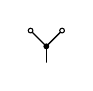
\begin{tikzpicture}[line cap=round,line join=round,>=triangle 45,x=0.2cm,y=0.2cm]
			\draw [line width=.5pt] (0.,0.)-- (0.,1.);
			\draw [line width=.5pt] (0.,1.)-- (-1.,2.);
			\draw [line width=.5pt] (0.,1.)-- (1.,2.);
			%marquages sommets
			\filldraw (0,1) circle(0.15);
			\draw[color=black, fill=white] (-1,2) circle (0.15);
			\draw[color=black, fill=white] (1,2) circle (0.15);
\end{tikzpicture}}}

\newcommand{\YY}{\raisebox{-0.3\height}{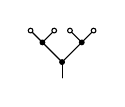
\begin{tikzpicture}[line cap=round,line join=round,>=triangle 45,x=0.2cm,y=0.2cm]
			\draw (0,0)--(0,1);
			\draw (0,1)--(-2,3);
			\draw (-1.25,2.25)--(-0.5,3);
			\draw (1.25,2.25)--(0.5,3);
			\draw (0,1)--(2,3);
			%marquage sommets
			\draw[color=black, fill=white] (-2,3) circle (0.15);
			\draw[color=black, fill=white] (2,3) circle (0.15);
			\draw[color=black, fill=white] (-0.5,3) circle (0.15);
			\draw[color=black, fill=white] (0.5,3) circle (0.15);
			\filldraw (0,1) circle(0.15);
			\filldraw (1.25,2.25) circle(0.15);
			\filldraw (-1.25,2.25) circle(0.15);
\end{tikzpicture}}}

\newcommand{\peignedroit}[3]{\raisebox{-0.5\height}{\begin{tikzpicture}[line cap=round,line join=round,>=triangle 45,x=0.25cm,y=0.25cm]
			% Etage 1
			\draw (0,0)--(0,1);
			%Etage 2
			\draw (0,1)--(-1,2) node[left]{${#1}$};
			% Etage 3
			\draw (0,1)--(6,7);
			\draw (2,3)--(1,4) node[left]{${#2}$};
			%Etage...
			\draw (3.,4.5) node[rotate=45]{$\cdots$};
			%Etage k
			\draw (5,6)--(4,7) node[left]{${#3}$};
			%marquage des sommets
			\filldraw (0,1) circle (0.15);
			\filldraw (2,3) circle (0.15);
			\filldraw (5,6) circle (0.15);
			\draw[color=black, fill=white](6,7) circle (0.15);
\end{tikzpicture} }}

\newcommand{\peignegauche}[3]{\raisebox{-0.5\height}{\begin{tikzpicture}[line cap=round,line join=round,>=triangle 45,x=0.25cm,y=0.25cm]
			% Etage 1
			\draw (0,0)--(0,1);
			%Etage 2
			\draw (0,1)--(1,2) node[right]{${#1}$};
			% Etage 3
			\draw (0,1)--(-6,7);
			\draw (-2,3)--(-1,4) node[right]{${#2}$};
			%Etage...
			\draw (-3.,4.5) node[rotate=135]{$\cdots$};
			%Etage k
			\draw (-5,6)--(-4,7) node[right]{${#3}$};
			%marquage des sommets
			\filldraw (0,1) circle (0.15);
			\filldraw (-2,3) circle (0.15);
			\filldraw (-5,6) circle (0.15);
			\draw[color=black, fill=white](-6,7) circle (0.15);
\end{tikzpicture}}}

\newcommand{\unitree}{\raisebox{-0.3\height}{\begin{tikzpicture}[line cap=round,line join=round,>=triangle 45,x=0.2cm,y=0.2cm]
		\draw (0,0)--(0,2);
		\filldraw[color=black,fill=white] (0,2) circle (0.15);
		\filldraw[color=black,fill=black] (0,0) circle (0.15);		
\end{tikzpicture}}}

\newcommand{\balais}{\raisebox{-0.3\height}{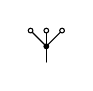
\begin{tikzpicture}[line cap=round,line join=round,>=triangle 45,x=0.2cm,y=0.2cm]
			\draw (0,0)--(0,2);
			\draw (0,1)-- (-1,2);
			\draw (0,1)-- (1,2);
			\filldraw[color=black, fill=white] (-1,2) circle(0.15);
			\filldraw[color=black, fill=white] (0,2) circle(0.15);
			\filldraw[color=black, fill=white] (1,2) circle(0.15);
			\filldraw[color=black] (0,1) circle(0.15);
\end{tikzpicture}}}
\newcommand{\balaisg}{\raisebox{-0.3\height}{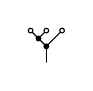
\begin{tikzpicture}[line cap=round,line join=round,>=triangle 45,x=0.2cm,y=0.2cm]
			\draw (0,0)-- (0,1);
			\draw (0,1)-- (-1,2);
			\draw (-0.5,1.5)-- (0,2);
			\draw (0,1)-- (1,2);
			\filldraw[color=black, fill=white] (-1,2) circle(0.15);
			\filldraw[color=black, fill=white] (0,2) circle(0.15);
			\filldraw[color=black, fill=white] (1,2) circle(0.15);
			\filldraw[color=black] (0,1) circle(0.15);
			\filldraw[color=black] (-0.5,1.5) circle(0.15);
\end{tikzpicture}}}
\newcommand{\balaisd}{\raisebox{-0.3\height}{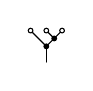
\begin{tikzpicture}[line cap=round,line join=round,>=triangle 45,x=0.2cm,y=0.2cm]
			\draw (0,0)-- (0,1);
			\draw (0,1)-- (-1,2);
			\draw (0.5,1.5)-- (0,2);
			\draw (0,1)-- (1,2);
			\filldraw[color=black, fill=white] (-1,2) circle(0.15);
			\filldraw[color=black, fill=white] (0,2) circle(0.15);
			\filldraw[color=black, fill=white] (1,2) circle(0.15);
			\filldraw[color=black] (0,1) circle(0.15);
			\filldraw[color=black] (0.5,1.5) circle(0.15);
\end{tikzpicture}}}
\DeclareDocumentCommand{\corollagraft}{m m m m}{\raisebox{-0.5\height}{\begin{tikzpicture}[line cap=round,line join=round,>=triangle 45,x=0.4cm,y=0.4cm]
			\draw (0,0)--(0,1);
			\draw (0,1)-- (-2,3) node[above,left] {$t_{#1}$};
			\draw (0,1)-- (-1,3) node[above] {$t_{#2}$};
			\draw (0,1)-- (1,3) node[above] {$t_{#3}$};
			\draw (0,1)-- (2,3) node[above,right] {$t_{#4}$};
			\draw (0,2.5) node[above] {$\dots$};
\end{tikzpicture}}}


%%%%%%%%%%%%%%%%%%%%%%%%%%%%%%%%%%%%%%%%%%%%%%%%%%%%%%%%%%%%%%%%%%%%%%%%%%%%%%%%%%%%%%%%%%%%%%%%%%%%%%%%%
%%%%%%%%%%%%%%%%%%%%% Macros d'édition pour laisser des commentaires %%%%%%%%%%%%%%%%%%%%%%%%%%%%%%%%%%%%%
%%%%%%%%%%%%%%%%%%%%%%%%%%%% ou montrer les changements %%%%%%%%%%%%%%%%%%%%%%%%%%%%%%%%%%%%%%%%%%%%%%%%%%
%%%%%%%%%%%%%%%%%%%%%%%%%%%%%%%%%%%%%%%%%%%%%%%%%%%%%%%%%%%%%%%%%%%%%%%%%%%%%%%%%%%%%%%%%%%%%%%%%%%%%%%%%%

%Pour les modifications

\NewEnviron{Jean}{{\color{red} \BODY }}
\NewEnviron{Pierre}{{\color{blue} \BODY }}
\NewEnviron{Loic}{{\color{olive} \BODY }}

% Macro faite pour supporter les sauts de lignes dans l'argument.

\newcommand{\JF}[1]{\begin{Jean}
		#1
\end{Jean}}
\newcommand{\PC}[1]{\begin{Pierre}
		#1
	\end{Pierre}{}}
\newcommand{\LF}[1]{\begin{Loic}
		#1
\end{Loic}}

%Pour les questions et remarque sur l'édition
% Attention, ne supporte pas les sauts de lignes dans l'argument.

\newcommand{\PCt}[1]{{\color{blue} \texttt{#1}}}
\newcommand{\JFt}[1]{{\color{red} \texttt{#1}}}
\newcommand{\LFt}[1]{{\color{olive} \texttt{#1}}}

\begin{document}

\maketitle

\begin{abstract}
	We introduce a primitive computation problem in the free tridendriform algebra generated by one element which is a Hopf algebra based on \Schw{} trees. We know a complex way to generate all of them, hence we want to implement this method on a computer. However, we need to create some tools to implement Schroeder trees and the multiplications over this algebra to be able to compute the primitive elements. In this paper, we detail how we made the problem mathematically understandable for a computer and how we did implement it.
\end{abstract}

\section{Introduction}

\subsection{Aim and structure of the paper}

The objective of this work  is to implement the objects and operations in a Hopf algebra involving \Schw{} trees. Those trees introduced in definition~\ref{defi:Sch_tree} can be endowed with three linear maps $\prec, \succ$ and $\cdot$ making it a free tridendriform algebra structure~\cite{LodayRonco_98,Catoire_2023, Manchon_2020} where the products can be described with quasi-shuffles (theorem~\ref{thm:produit}) . 
Tridendriform algebras arise in different topics in mathematics like free probability~\cite{Celestino_2022, Ebrahimi-Fard_Patras_2018}, the study of Rota-Baxter algebras~\cite{Manchon_RB_2020, Gao_2019} or in other topics like number theory~\cite{Ho00, Catoire_2025}.
Some computation tools already exist for some algebras on \Sage{}~\cite{Sage_book,Sage_doc} but not for all. 
Hence, implementing the free tridendriform algebra~\cite{Catoire_2023} (over one generator) allows us to implement any tridendriform algebras coding a quotient map by a tridendriform ideal from \Schw{} trees to the desired objects.

This algebra turns out to be a Hopf algebra with its coproduct given in theorem~\ref{thm:coproduit}. Computing the space of primitive elements of this algebra, we describe at least the largest cocommutative algebra inside it thanks to the Cartier-Quillen-Milnor-Moore theorem~\cite{May_69,MilnorMoore_65, CartierPatras_2021}. An inductive algorithm is given in the article~\cite{Catoire_2023} (shown in figure~\ref{fig:algo_idea}) to compute those elements using only $\prec, \succ$ and $\cdot$ operations.  

Initially, we wanted to implement efficiently (i.e  with low complexity) this algorithm to compute all primitive elements in any degree.
But to our surprise, using some naive approaches, this task is really difficult. Hence, we need to choose a point of view of the problem to get a clear and efficient implementation of this algorithm. 

To solve this problem, we used a particular representations of \Schw{} trees as initial chains (definition~\ref{def:init_chain}) or specific sequences over the alphabet $\{0,1\}$ (definition~\ref{defi:lifetime}). Those representations are called \emph{codes} of the tree. Thanks to this point of view, we are able to describe the action of quasi-shuffles on a pair of codes in definition~\ref{defi:quasishuffle_code} such that it describes the initial action of these elements onto a pair of \Schw{} trees (theorem~\ref{Cor:iso_codes_trees}). We present the implementation in {\ttfamily  C++} of the trees as codes and of the three basics operations $\prec, \succ$ and $\cdot$ on codes that are equivalent to the original ones on \Schw{} trees. We evaluate its time and memory complexity.


The paper is divided in the following way:
\begin{itemize}
	\item Section~\ref{sec:the_problem} describes and gives the minimum piece of information needed to understand the general mathematical setting in which we are working. We introduce the main objects of this work, \Schw{} trees in definition~\ref{defi:Sch_tree} and quasi-shuffles in definition~\ref{def:quasi_shuffles}. Then, we detail the Hopf algebra structure on $(\K\Sch,\prec, \succ, \cdot)$ (figure~\ref{fig:algo_idea}) and we introduce the algorithm which computes its space of primitive elements.
	\item Section~\ref{sec:pov} is a mathematical description of the encoding used to implement our problem. We introduce the concept of \Schw{} levelled trees (definition~\ref{defi:levelled_trees}), initial chains and the map associating to any initial chain a $0$'s  and $1$'s sequence (definition~\ref{def:init_chain}). Then, we choose a way to map any \Schw{} tree to a levelled \Schw{} tree (proposition~\ref{prop:trees_to_levels}) which gives a way to get a $0$'s and $1$'s	sequence from any \Schw{} tree. A sequence obtained by this transformation will be called a \emph{tree code}. Finally, we present a tridendriform structure on tree codes (definition~\ref{defi:quasishuffle_code}) that turns out to be isomorphic to the one on \Schw{} trees (corollary~\ref{Cor:iso_codes_trees}).
	\item The last section~\ref{sec:coding} explains the implementation we made in {\ttfamily C++} to perform some computations and the results it produces. 
\end{itemize}


\subsection{Notations used in the article}

In this list, we put a table of contents of notations used here :
\begin{itemize} %TODO To update
	\item for any $n\in\NN^*, \IEM{1}{n}$ is the set $\{1,\dots, n\}$;
	\item for any set $X$, we denote by $\K X$ the vector space over $\K$ whose basis is $X$;
	\item for any set $X$, we denote $\Par(X)$ the set of its subsets. It is endowed with the refinement order $\leq_{\pi}$;
	\item for any set $X, X^{\star}$ denotes the set of finite words over the alphabet $X$. We denote by $T(\K X)$ the $\K$-vector space whose basis is $X^{\star}$;
	\item for any graded set $X=\bigoplus_{n=0}^{+\infty} X_n,$ for any $n\in\NN$, we define $T(\K X)(n)$ the subspace whose basis is the set $X^{\star}$ where the sum of the degree's of its letters is $n$; 
	\item $(\K\Sch, \pleft, \pmid, \pright)$ the graded tridendriform algebra on Schroeder tree;
	\item $\Sch(\nn)$ the set of Schroeder tree with $\nn$ leaves;
	\item $\SchF$ the set of forest of Schroeder tree;
	\item $\vee$ is the grafting operator of many trees onto a common root;
	\item given a sequence $x=(x_1,\dots, x_n)$ and $i\in\IEM{1}{n},$ we denote by $x\setminus (x_i)$ the sequence $x$ without the term $x_i$;
	\item for reasons of length some increasing sequences will be written in columns. Doing so the minimal element of the sequence is a the bottom of the column representation of the sequence.
\end{itemize}

\subsection{Acknowledgments}

The authors would like to thank LMPA of ULCO for welcoming me during this collaboration.

\section{About the original problem} \label{sec:the_problem}

\subsection{\Schw{} trees and comb representations}

Let us remind the following definition:
\begin{defi}\label{defi:Sch_tree}
	A \emph{\Schw{} tree} is a planar rooted tree such that any vertices which is not a leaf has at least $2$ children.
	This set can be graded with the number of leaves minus $1$. For any $n\in\NN\setminus\{0\}$, we define $\Sch(\nn)$ the set of \Schw{} trees with $n+1$ leaves.
	We also put $\Sch(0)=\left\{\unitree\right\}$ and define: 
	\[
	\Sch\coloneqq \bigcup_{n=0}^{+\infty} \Sch(\nn) \text{ and } \overline{\Sch}=\bigcup_{n=1}^{+\infty} \Sch(\nn).
	\]
	Given any $t\in\Sch,$ we will denote $V(t)$ the set of vertices which are not leaves and $E(t)$ its set of edges. We call them \emph{internal vertices} of $t$. In the sequel, they are drawn as black disks.
\end{defi}
\begin{exam}\label{exam:Sch3} %Attention, c'est 3 ici, \Sch(n) c'est les arbres à n+1 feuilles.
	The elements of $\Sch(3)$ are
	\vspace{0.5em}
	\begin{center}
		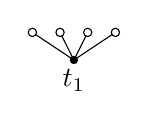
\begin{tikzpicture}[x=1em,y=1em]
			\draw(-1.5,1) -- (0,0);
			\draw(-0.5,1) -- (0,0);
			\draw(0.5,1) -- (0,0);
			\draw(1.5,1) -- (0,0);
			\draw[color=black, fill=white](-1.5,1) circle(0.15);
			\draw[color=black, fill=white](-0.5,1) circle(0.15);
			\draw[color=black, fill=white](0.5,1) circle(0.15);
			\draw[color=black, fill=white](1.5,1) circle(0.15);
			\fill(0,0) circle(0.15) node[below]{$t_1$};
		\end{tikzpicture}
		\hspace{1em}
		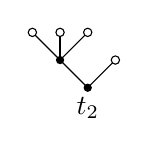
\begin{tikzpicture}[x=1em,y=1em]
			\draw(-1,2) -- (0,1);
			\draw(0,2) -- (0,1);
			\draw(1,2) -- (0,1);
			\draw(2,1) -- (1,0);
			\draw(0,1) -- (1,0);
			\draw[color=black, fill=white](-1,2) circle(0.15);
			\draw[color=black, fill=white](0,2) circle(0.15);
			\draw[color=black, fill=white](1,2) circle(0.15);
			\draw[color=black, fill=white](2,1) circle(0.15);
			\fill(1,0) circle(0.15) node[below]{$t_2$};
			\fill (0,1) circle(0.15);
		\end{tikzpicture}
		\hspace{1em}
		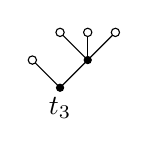
\begin{tikzpicture}[x=1em,y=1em]
			\draw(-1,1) -- (0,0);
			\draw(0,2) -- (1,1);
			\draw(1,2) -- (1,1);
			\draw(2,2) -- (1,1);
			\draw(1,1) -- (0,0);
			\draw[color=black, fill=white](-1,1) circle(0.15);
			\draw[color=black, fill=white](0,2) circle(0.15);
			\draw[color=black, fill=white](1,2) circle(0.15);
			\draw[color=black, fill=white](2,2) circle(0.15);
			\fill(0,0) circle(0.15) node[below]{$t_3$};
			\fill (1,1) circle(0.15);
		\end{tikzpicture}
		\hspace{1em}
		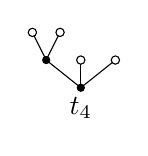
\begin{tikzpicture}[x=1em,y=1em]
			\draw(1,1) -- (-0.25,0);
			\draw(-0.25,1) -- (-0.25,0);
			\draw(-1,2) -- (-1.5,1);
			\draw(-2,2) -- (-1.5,1);
			\draw(-1.5,1) -- (-0.25,0);
			\draw[color=black, fill=white](1,1) circle(0.15);
			\draw[color=black, fill=white](-0.25,1) circle(0.15);
			\draw[color=black, fill=white](-1,2) circle(0.15);
			\draw[color=black, fill=white](-2,2) circle(0.15);
			\fill(-0.25,0) circle(0.15) node[below]{$t_4$};
			\fill (-1.5,1) circle(0.15);
		\end{tikzpicture}
		\hspace{1em}
		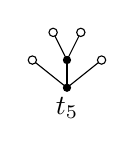
\begin{tikzpicture}[x=1em,y=1em]
			\draw(-0.25,2) -- (0.25,1);
			\draw(0.75,2) -- (0.25,1);
			\draw(-1,1) -- (0.25,0);
			\draw(0.25,1) -- (0.25,0);
			\draw(1.5,1) -- (0.25,0);
			\draw[color=black, fill=white](-1,1) circle(0.15);
			\draw[color=black, fill=white](-0.25,2) circle(0.15);
			\draw[color=black, fill=white](0.75,2) circle(0.15);
			\draw[color=black, fill=white](1.5,1) circle(0.15);
			\fill(0.25,0) circle(0.15) node[below]{$t_5$};
			\fill (0.25,1) circle(0.15);
		\end{tikzpicture}
		\hspace{1em}
		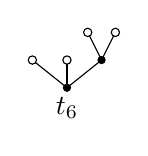
\begin{tikzpicture}[x=1em,y=1em]
			\draw(-1,1) -- (0.25,0);
			\draw(0.25,1) -- (0.25,0);
			\draw(1,2) -- (1.5,1);
			\draw(2,2) -- (1.5,1);
			\draw(1.5,1) -- (0.25,0);
			\draw[color=black, fill=white](-1,1) circle(0.15);
			\draw[color=black, fill=white](0.25,1) circle(0.15);
			\draw[color=black, fill=white](1,2) circle(0.15);
			\draw[color=black, fill=white](2,2) circle(0.15);
			\fill(0.25,0) circle(0.15) node[below]{$t_6$};
			\fill (1.5,1) circle(0.15);
		\end{tikzpicture}
		\vspace{1em}
	\end{center}
	\begin{center}
		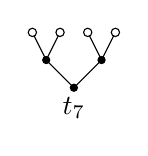
\begin{tikzpicture}[x=1em,y=1em]
			\draw(0,2) -- (0.5,1);
			\draw(1,2) -- (0.5,1);
			\draw(2,2) -- (2.5,1);
			\draw(3,2) -- (2.5,1);
			\draw(0.5,1) -- (1.5,0);
			\draw(2.5,1) -- (1.5,0);
			\draw[color=black, fill=white](0,2) circle(0.15);
			\draw[color=black, fill=white](1,2) circle(0.15);
			\draw[color=black, fill=white](2,2) circle(0.15);
			\draw[color=black, fill=white](3,2) circle(0.15);
			\fill(1.5,0) circle(0.15) node[below]{$t_7$};
			\fill (0.5,1) circle(0.15);
			\fill (2.5,1) circle(0.15);
		\end{tikzpicture}
		\hspace{1em}
		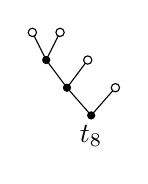
\begin{tikzpicture}[x=1em,y=1em]
			\draw(-1,2) -- (-0.5,1);
			\draw(0,2) -- (-0.5,1);
			\draw(1,1) -- (0.25,0);
			\draw(-0.5,1) -- (0.25,0);
			\draw(0.25,0) -- (1.125, -1);
			\draw(2,0) -- (1.125, -1);
			\draw[color=black, fill=white](-1,2) circle(0.15);
			\draw[color=black, fill=white](0,2) circle(0.15);
			\draw[color=black, fill=white](1,1) circle(0.15);
			\draw[color=black, fill=white](2,0) circle(0.15);
			\fill(1.125,-1) circle(0.15) node[below]{$t_8$};
			\fill (0.25,0) circle(0.15);
			\fill (-0.5,1) circle(0.15);
		\end{tikzpicture}
		\hspace{1em}
		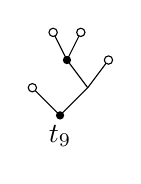
\begin{tikzpicture}[x=1em,y=1em]
			\draw(-1,2) -- (-0.5,1);
			\draw(0,2) -- (-0.5,1);
			\draw(1,1) -- (0.25,0);
			\draw(-0.5,1) -- (0.25,0);
			\draw(0.25,0) -- (-0.75,-1);
			\draw(-1.75,0) -- (-0.75,-1);
			\draw[color=black, fill=white](-1,2) circle(0.15);
			\draw[color=black, fill=white](0,2) circle(0.15);
			\draw[color=black, fill=white](1,1) circle(0.15);
			\draw[color=black, fill=white](-1.75,0) circle(0.15);
			\fill(-0.75,-1) circle(0.15) node[below]{$t_9$};
			\fill (-0.5,1) circle(0.15);
		\end{tikzpicture}
		\hspace{1em}
		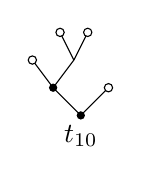
\begin{tikzpicture}[x=1em,y=1em]
			\draw(1,2) -- (0.5,1);
			\draw(0,2) -- (0.5,1);
			\draw(-1,1) -- (-0.25,0);
			\draw(0.5,1) -- (-0.25,0);
			\draw(-0.25,0) -- (0.75,-1);
			\draw(1.75,0) -- (0.75,-1);
			\draw[color=black, fill=white](1,2) circle(0.15);
			\draw[color=black, fill=white](0,2) circle(0.15);
			\draw[color=black, fill=white](-1,1) circle(0.15);
			\draw[color=black, fill=white](1.75,0) circle(0.15);
			\fill(0.75,-1) circle(0.15) node[below]{$t_{10}$};
			\fill (-0.25,0) circle(0.15);
		\end{tikzpicture}
		\hspace{1em}
		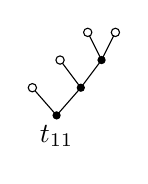
\begin{tikzpicture}[x=1em,y=1em]
			\draw(1,2) -- (0.5,1);
			\draw(0,2) -- (0.5,1);
			\draw(-1,1) -- (-0.25,0);
			\draw(0.5,1) -- (-0.25,0);
			\draw(-0.25,0) -- (-1.125, -1);
			\draw(-2,0) -- (-1.125, -1);
			\draw[color=black, fill=white](1,2) circle(0.15);
			\draw[color=black, fill=white](0,2) circle(0.15);
			\draw[color=black, fill=white](-1,1) circle(0.15);
			\draw[color=black, fill=white](-2,0) circle(0.15);
			\fill(-1.125,-1) circle(0.15) node[below]{$t_{11}$};
			\fill (-0.25,0) circle(0.15);
			\fill (0.5,1) circle(0.15);
		\end{tikzpicture}.
	\end{center}
\end{exam}


% N'est plus pertinent
%\begin{Rq}
%	For theses trees, as every node which is not a leaf has at least $2$ children we will not draw the nodes of a tree any more.
%\end{Rq}

Let $t$ be a tree. It can always be seen as a comb:
\begin{center}
	\raisebox{-0.5\height}{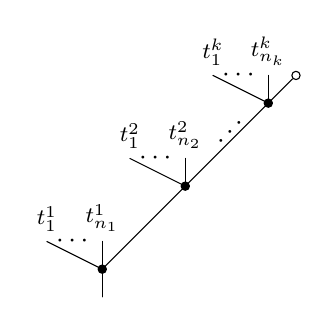
\begin{tikzpicture}[line cap=round,line join=round,x=1em,y=1 em]
			% Etage 1
			\draw (0,0)--(0,1);
			\filldraw (0,1) circle (0.15);
			%Etage 2
			\draw (0,1)--(-2,2)
			 node[above]{\footnotesize{$t^1_1$}};
			\draw (0,1)--(0,2) node[above]{\footnotesize{$t^1_{n_1}$}};
			\draw (-1,2) node{$\cdots$};
			% Etage 3
			\draw (0,1)--(7,8);
			\filldraw[color=white] (7,8) circle (0.15);
			\draw (3,4)--(1,5) node[above]{\footnotesize{$t^2_1$}};
			\filldraw (3,4) circle (0.15);
			\draw (3,4)--(3,5) node[above]{\footnotesize{$t^2_{n_2}$}};
			\draw (2,5) node{$\cdots$};
			%Etage...
			\draw (4.7,6) node[rotate=45]{$\cdots$};
			%Etage k
			\draw[color=black, fill=white](7,8) circle(0.15);
			\filldraw (6,7) circle (0.15);
			\draw (6,7)--(4,8) node[above]{\footnotesize{$t^k_1$}};
			\draw (6,7)--(6,8) node[above]{\footnotesize{$t^k_{n_k}$}};
			\draw (5,8) node {$\cdots$};
	\end{tikzpicture}},
\end{center}
where $k$ is the number of nodes on the right-most branch of $t$ and for $i\in\IEM{1}{k}, n_i+1$ is the number of sons of the $i$-th node of this branch.

\begin{Not}
	Let $F=t_1\dots t_n$ be a forest composed of $n$ trees. For simplicity, we write 
	\raisebox{-0.3\height}{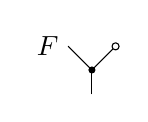
\begin{tikzpicture}[line cap=round,line join=round,x=0.3cm,y=0.3cm]
			% Etage 1
			\draw (0,0)--(0,1);
			%Etage 2
			\draw (0,1)--(-1,2) node[left]{$F$};
			\draw (0,1)--(1,2);
			\draw[color=black, fill=white] (1,2) circle (0.15);
			\fill (0,1) circle(0.15);
	\end{tikzpicture}} instead of:
	\begin{center}
		\raisebox{-0.5\height}{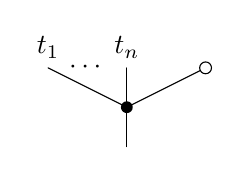
\begin{tikzpicture}[line cap=round,line join=round,x=0.5cm,y=0.5cm]
				% Etage 1
				\draw (0,0)--(0,1);
				%Etage 2
				\draw (0,1)--(-2,2) node[left,above]{$t_1$};
				\draw (0,1)--(0,2) node[right,above]{$t_{n}$};
				\draw (-1,2) node{$\cdots$};
				\draw (0,1)--(2,2);
				\draw[color=black, fill=white] (2,2) circle (0.15);
				\fill (0,1) circle(0.15);
		\end{tikzpicture}}.
	\end{center}
\end{Not}

With these notations, we notice that all tree $t$ can be seen either respectively like a \emph{right comb} or a \emph{left comb}:
\begin{align}\label{eq:tree_combs}
	t&=\peignedroit{F_1}{F_2}{F_k}
	& \text{ and } &&  t=\peignegauche{F_{k+1}}{F_{k+2}}{F_{k+l}},
\end{align}
where $F_1,\dots,F_k$ and $F_{k+1},\dots, F_{k+l}$ are non-empty forests.
\begin{defi}
	The writing defined above at the right	 is the writing of $t$ as a \emph{right comb}.
	Proceeding the same way, looking at the left branch of the root of $t$, we get the writing of $t$ as a \emph{left comb}.
\end{defi}


\subsection{Our objective}

We describe the structure of bialgebra onto $\K\Sch$ and we explain how to compute its primitive elements thanks to some results~\cite{Catoire_2023,euleridem}.

\begin{defi}\label{def:tridend}
	Let $\K$ be a field and $A$ be vector space of $\K$. We say $(A,\prec,\cdot,\succ)$ is a \emph{tridendriform algebra} if $\prec,\cdot$ and $\succ$ are three linear maps from $A\otimes A$ to $A$ such that for any $a,b,c\in A$:
	\begin{align}
		(a\prec b)\prec c&=a\prec(b*c), \label{eq:tri1}\\
		(a\succ b)\prec c&=a\succ(b\prec c), \label{eq:tri2} \\
		(a* b)\succ c&=a\succ(b\succ c),  \label{eq:tri3} \\
		(a\succ b)\cdot c&=a\succ(b\cdot c), \label{eq:tri4} \\
		(a\prec b)\cdot c&=a\cdot(b\succ c), \label{eq:tri5} \\
		(a\cdot b)\prec c&=a\cdot(b\prec c), \label{eq:tri6} \\
		(a\cdot b)\cdot c&=a\cdot (b\cdot c), \label{eq:tri7}
	\end{align}
	where $*$ is the \emph{associative product} of the tridendriform algebra defined for any $a,b\in A$ by $a*b\coloneqq a\prec b + a\cdot b +a\succ b$. 
	We call the products $\succ,\prec,\cdot$ respectively right, left and middle.
\end{defi} 

The free tridendriform algebra is built on the vector space $\K\overline{\Sch}.$ We then add a unit $\unitree$ to the product $*$ by hand to get an algebra over $\K\Sch\oplus \K\cdot \unitree=\K\Sch$. We will denote it by $(\Sch{},\prec,\cdot,\succ)$. We have a combinatorial interpretation of the product $*$. For this let us introduce:
\begin{defi}[Quasi-shuffle]\label{def:quasi_shuffles}
	Let $k,l\in\NN\setminus \{0\}$. A \emph{$(k,l)$-quasi-shuffle} is a surjective map $\sigma:\IEM{1}{k+l}\twoheadrightarrow\IEM{1}{n}$ for some positive integer $n$
	such that:
	\[
	\sigma(1)<\cdots<\sigma(k) \text{  and  } \sigma(k+1)<\cdots<\sigma(k+l).
	\]
	We will denote $\batc(k,l)$ the set of all $(k,l)$-quasi-shuffles.
\end{defi}
We can easily prove that: %TODO ON ajoute une référence ou on le démontre ? Personnelemnt je pense qu'ajouter une référence est suffisant.
\begin{Lemma}\label{lem:Indution_batc}
	Let $k,l\geq 2$. Then, the following sets are in bijections:
	\begin{align*}
		\{\sigma\in\batc(k,l) \,|\, \sigma^{-1}(\{1\})=\{1\}\} &\simeq \batc(k-1,l), \\
		\{\sigma\in\batc(k,l) \,|\, \sigma^{-1}(\{1\})=\{k+1\}\} &\simeq \batc(k,l-1), \\
		\{\sigma\in\batc(k,l) \,|\, \sigma^{-1}(\{1\})=\{1,k+1\}\} &\simeq \batc(k-1,l-1).
	\end{align*}
	For other cases, we have:
	\[ % font issue for the and here
	\batc(1,0)=\{\Id_{\{1\}}\}=\batc(0,1) \text{ \textrm{and} } \batc(1,1)=\{\Id_{\{1,2\}}, (2,1)\}.
	\]
\end{Lemma}
\begin{proof}
	Let $k,l$ be two integers greater or equal to $2$.
	\begin{description}
		\item[First case] we denote by $\sigma':\IEM{1}{k+l-1}\rightarrow \NN$ the unique map such that:
		\[
		\forall n\in\IEM{1}{k+l}, \sigma(n)=\begin{cases}
			1 &\text{if } n=1, \\
			\sigma'(n-1)+1 & \text{otherwise.}
		\end{cases}
		\]
		It is left to the reader to check that $\sigma'$ is an element of $\batc(k-1,l).$
		\item[Second case] we denote by $\sigma':\IEM{1}{k+l-1}\rightarrow \NN$ the unique map such that:
		\[
		\forall n\in\IEM{1}{k+l}, \sigma(n)=\begin{cases}
			1 &\text{ if } n=k+1, \\
			\sigma'(n)+1 & \text{if } n<k+1, \\
			\sigma'(n-1)+1 & \text{otherwise.}
		\end{cases}
		\]
		It is left to the reader to check that $\sigma'$ is an element of $\batc(k,l-1).$
		\item[Third case] we denote $\sigma':\IEM{1}{k+l-1}\rightarrow \NN$ the unique map such that:
		\[
		\forall n\in\IEM{1}{k+l}, \sigma(n)=\begin{cases}
			1 &\text{ if } n=1 \text{ or } n=k+1, \\
			\sigma'(n-1)+1 & \text{ if } n\leq k, \\
			\sigma'(n-2)+1 & \text{ otherwise}. \\
		\end{cases}
		\]
		It is left to the reader to check that $\sigma'$ is an element of $\batc(k-1,l-1).$
	\end{description}
	Hence it establishes the maps from the left to the right in the lemma. Conversely, one remarks in any case that the map $\sigma\mapsto\sigma'$ is invertible.
\end{proof}


Let $t,s$ two trees different from $\unitree$. We look $t$ as a right comb and $s$ as a left comb. In other words, we put:
\begin{align}\label{eq:comb_ts}
	t&=\peignedroit{F_1}{F_2}{F_k}
	& \text{ and } &&  s=\peignegauche{F_{k+1}}{F_{k+2}}{F_{k+l}},
\end{align}
where for all $i\in\IEM{1}{k+l}, F_i$ is a non-empty forest. Here, $k$ represents the number of nodes on the right-most branch of $t$ and $l$ is the number of nodes on the left-most branch of $s$.

\begin{defi}\label{def:quasiaction}
	Let $t$ and $s$ be two trees which respective right comb representation and left comb representation are given above (equation~\eqref{eq:comb_ts}).
	We denote by $k$ (respectively $l$) the number of nodes on the right-most (respectively left-most) branch of $t$ (respectively $s$). Let $\sigma$ be a $(k,l)$-quasi-shuffle which has for image $\IEM{1}{n}$ with $n$ a non-negative integer. We denote $\sigma(t,s)$ the tree obtained this way:
	\begin{enumerate}
		\item  We first consider the ladder with $n$ nodes:
		\begin{center}
			\raisebox{-0.5\height}{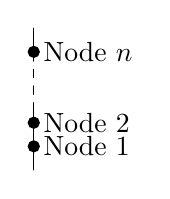
\begin{tikzpicture}[line cap=round,line join=round,>=triangle 45,x=0.3cm,y=0.3cm]
					\begin{scope}{shift={(-3,0)}}
						\draw (0,0)--(0,2.5);
						\draw[dashed] (0,2.5)--(0,5);
						\draw (0,5)--(0,6);
						\filldraw [black] (0,1) circle (2pt) node[anchor=west]{Node $1$};
						\filldraw [black] (0,2) circle (2pt) node[anchor=west]{Node $2$};
						\filldraw [black] (0,5) circle (2pt) node[anchor=west]{Node $n$};
					\end{scope}
			\end{tikzpicture}}.
		\end{center}
		\item For all $i\in\IEM{1}{k},$ we graft $F_i$ as the \emph{left} son at the node $\sigma(i)$.
		\item For all $i\in\IEM{k+1}{k+l},$ we graft $F_i$ as \emph{right} son at the node $\sigma(i)$.
	\end{enumerate}
\end{defi}

\begin{exam}\label{exam:quasiaction}
	Consider the $(2,2)$-quasi-shuffle $\sigma=(1,3,2,3)$.
	
	 Let us take 
	$t=$	\raisebox{-0.3\height}{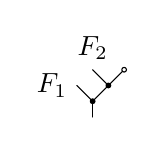
\begin{tikzpicture}[line cap=round,line join=round,>=triangle 45,x=0.2cm,y=0.2cm]
			% Etage 1
			\draw (0,0)--(0,1);
			%Etage 2
			\draw (0,1)--(-1,2) node[left]{$F_1$};
			% Etage 3
			\draw (0,1)--(2,3);
			\draw (1,2)--(0,3) node[left,above]{$F_2$};
			%marquages des sommets
			\filldraw (0,1) circle (0.15);
			\filldraw (1,2) circle (0.15);
			\draw[color=black, fill=white] (2,3) circle (0.15);
	\end{tikzpicture}} and $s=\raisebox{-0.3\height}{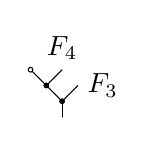
\begin{tikzpicture}[line cap=round,line join=round,>=triangle 45,x=0.2cm,y=0.2cm]
			% Etage 1
			\draw (0,0)--(0,1);
			%Etage 2
			\draw (0,1)--(1,2) node[right]{$F_{3}$};
			% Etage 3
			\draw (0,1)--(-2,3);
			\draw (-1,2)--(0,3) node[right,above]{$F_{4}$};
			%marquages des sommets
			\filldraw (0,1) circle (0.15);
			\filldraw (-1,2) circle (0.15);
			\draw[color=black, fill=white] (-2,3) circle (0.15);
	\end{tikzpicture}}$.
	Then $\sigma(t,s)=$\raisebox{-0.5\height}{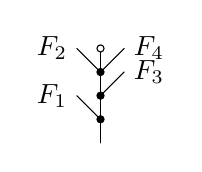
\begin{tikzpicture}[line cap=round,line join=round,>=triangle 45,x=0.3cm,y=0.3cm]
			\draw (0,0)--(0,4);
			%Noeud 1
			\draw (0,1)--(-1,2) node[left]{$F_1$};
			%Noeud 2
			\draw (0,2)--(1,3) node[right]{$F_3$};
			%Noeud 3
			\draw (0,3)--(-1,4) node[left]{$F_2$};
			\draw (0,3)--(1,4) node[right]{$F_4$};
			%marquage des noeuds
			\filldraw (0,1) circle (0.15);
			\filldraw (0,2) circle (0.15);
			\filldraw (0,3) circle (0.15);
			\draw[color=black, fill=white] (0,4) circle (0.15);
	\end{tikzpicture}}.
\end{exam} 

\begin{thm}[\cite{Catoire_2023}]\label{thm:produit}
	Let $t,s$ be two trees different from $\unitree$ as described above. Then: 
	\[
	t*s=\sum_{\sigma\in \batc(k,l)}\sigma(t,s).
	\]
	Moreover:
	\begin{gather*}
		t\prec s=\sum_{\substack{\sigma\in\batc(k,l) \\ \sigma^{-1}(\{1\})=\{1\}}} \sigma(t,s), 
		 t\succ s=\sum_{\substack{\sigma\in\batc(k,l) \\ \sigma^{-1}(\{1\})=\{k+1\}}} \sigma(t,s),\\
		t\cdot s=\sum_{\substack{\sigma\in\batc(k,l) \\ \sigma^{-1}(\{1\})=\{1,k+1\}}} \sigma(t,s).
	\end{gather*}
\end{thm}
This result is a combinatorial description of an inductive formula given in the previous work of J.L.~Loday and M.~Ronco~\cite{LodayRonco_98}.
Surprisingly,  $(\K\Sch,\prec,\cdot,\succ)$ can be endowed with a codendriform coproduct~\cite{Catoire_2023,LodayRonco_98}:
\begin{thm}\label{thm:coproduit}
	We define a map $\Delta:\K\Sch\rightarrow \K\Sch\otimes \K\Sch$ by:
	\begin{align*}
		\Delta(t)=\sum_{c \text{ \normalfont admissible cut of }t} P^c(t)\otimes R^c(t),
	\end{align*}
	where $R^c(t)$ is the component of $t$ containing its root and $P^c(t)=P^c_1(t)*\cdots *P^c_k(t)$, where $P^c_i(t)$ are the cut trees naturally ordered from left to right. Moreover one can write $\Delta=\Delta_{\leftarrow}+\Delta_{\rightarrow}$ in such a way so $(\K\Sch,\prec,\cdot,\succ,\Delta_{\leftarrow},\Delta_{\rightarrow})$ is a $(3,2)$-dendriform bialgebra detailled in~\cite{Catoire_2023}.
\end{thm}

From the Cartier-Quillen-Milnor-Moore theorem~\cite{CartierPatras_2021}, we can understand better the cocommutative part of this Hopf algebra from its primitives.
Hence, a natural question is to compute the primitive elements of $\K\Sch$. Let us introduce the notations to reach the theorems for this purpose:
\begin{defi}
	Let $(C,\Delta_{\leftarrow},\Delta_{\rightarrow})$ be a dendriform coalgebra. We define:
	\begin{gather*}
		\Prim_{\leftarrow}(C):=\{ c\in C \,|\, \tilde{\Delta}_{\leftarrow}(c)=0 \}, 
		\Prim_{\rightarrow}(C):=\{ c\in C \,|\, \tilde{\Delta}_{\rightarrow}(c)=0 \}, \\
		\Prim_{\Coass}(C):=\{ c\in C \,|\, \tilde{\Delta}(c)=0 \},
		\Prim_{\Codend}(C):=\{ c\in C \,|\, \tilde{\Delta}_{\leftarrow}(c)=\tilde{\Delta}_{\rightarrow}(c)=0 \}.
	\end{gather*}
\end{defi}

In particular, with respect to the grading of $\Sch$, we have:
\begin{align*}
	& \Prim_{\Coass}(\K\Sch(1))=\left\langle\Y\right\rangle, &\Prim_{\Codend}(\K\Sch(1))=\left\langle\Y\right\rangle, \\
	& \Prim_{\Coass}(\K\Sch(2))=\left\langle \balais, \balaisd - \balaisg \ \right\rangle, & \Prim_{\Codend}(\K\Sch(2))=\left\langle \balais \right\rangle.
\end{align*}
\begin{thm}[\cite{Catoire_2023}]\label{thm:coassincodend}
	For all $n\in\NN$, we define:
	\begin{equation*}
		\theta_n:\left\lbrace \begin{array}{rcl}
			\Prim_{\Coass}(\K\Sch(n))& \rightarrow & \Prim_{\Codend}(\K\Sch(n+1)), \\
			a\otimes \Y & \mapsto & a\cdot \Y.
		\end{array}\right.
	\end{equation*}
	Then, for all $n\in\NN, \theta_n$ is an isomorphism of vector spaces.
\end{thm}
Let us introduce for any $n\in\NN$, the vector space:
\[
W_n=\Prim_{\Codend}(\K\Sch)_n \oplus \left\langle w \, \middle| \, w\in T^k(\Prim_{\Coass}(\K\Sch))(n) \text{ with } k>1 \right\rangle,
\]
where $T^k(V)$ is the vector space generated by words of length exactly $k$.
From the article~\cite{euleridem} of M.~Ronco, we find an analogous of the following theorem~\ref{thm:coassincodend} in terms of \emph{brace algebras}. We state it in a simpler way in exchange of a loss of injectivity:
\begin{thm}\label{thm:génération2}
	 One can define  a map $\omega$ using $\pright,\pmid$ and $\pleft$ giving rise for all $n\in\NN$ to:
	\begin{equation}\label{eq:Omega}
		\Omega_n:\left\lbrace\begin{array}{rcl}
			T(\Prim_{\Coass}(\K\Sch))(n) & \twoheadrightarrow & \Prim_{\Coass}(\K\Sch(n)), \\
			x_1\otimes\dots\otimes x_k & \mapsto & \omega(x_1\otimes \dots \otimes x_k).
		\end{array}\right.
	\end{equation}
	This raise to a map $\Omega$ defined over $\Sch$ such that $\Omega|_{T(\Prim_{\Codend}(\K\Sch(n)))}=\Omega_n$. The map $\omega$ is defined for any $k\geq 2, x,y,x_1,\dots, x_k\in\K\Sch$ by:
	\begin{align*}
		&\omega(x)\coloneqq x, \\ 
		&\omega(x_1\otimes \ldots \otimes x_k \otimes y)= \sum_{i=0}^k (-1)^{k-i} \omega_{\prec}(x_1\otimes\ldots \otimes x_i) \succeq y \prec \omega_{\succeq}(x_{i+1}\otimes \ldots \otimes x_k),
	\end{align*}
	where:
	\begin{align*}
		&\omega_{\prec}(\ew)=\unitree = \omega_{\succ}(\ew), \\
		&\omega_{\prec}(x_1\otimes \ldots \otimes x_k)= x_1\prec \omega_{\prec}(x_2\otimes \ldots \otimes x_k), \\
		&\omega_{\succeq}(x_1\otimes \ldots \otimes x_k)= \omega_{\succeq}(x_1\otimes \ldots \otimes x_{k-1})\succeq x_k.
	\end{align*}
\end{thm}

\begin{exam}
	To compute an element of $\Prim_{\Coass}(\K\Sch(3))$, we can choose $\Y\otimes \Y \otimes \Y$ or $\left(\balaisd - \balaisg\right) \otimes \Y$ which are both elements of $T^{\leq 2}(\K\Prim_{\Coass})(3).$ Hence:
\begin{align*}
	\Omega_3\left(\Y\otimes \Y \otimes \Y\right)&= \Y \prec \left( \Y \succeq \Y\right) - \Y \succeq \Y \prec \Y + \left(\Y \prec \Y\right)\succeq \Y,\\
	\Omega_3\left( \left(\balaisd - \balaisg\right) \otimes \Y\right) &= - \Y\prec \left(\balaisd - \balaisg\right) + \left(\balaisd - \balaisg\right)\succeq \Y.
\end{align*} 	
\end{exam}

So, we have a recipe to produce the primitives of this algebra by induction as shown in figure~\ref{fig:algo_idea}:
%\begin{figure}[h]
%	\centering
%	\begin{tikzcd}
%		&
%		\Prim_{\Codend}(\K\Sch(1)) \ar[out=-20, in=160, "\Omega_1", swap]{dl} \\ 
%		 \Prim_{\Coass}(\K\Sch(2)) \arrow[r,"\theta_1"] & \Prim_{\Codend}(\K\Sch(2)) \ar[out=-20, in=160, swap, "\Omega_2"]{dl} \\
%		\Prim_{\Codend}(\K\Sch(3)) \arrow[r,"\theta_2"] & \dots 
%	\end{tikzcd}
%	\caption{Diagram of the induction}
%	\label{fig:algo_idea0}
%\end{figure}
\begin{figure}[h]
	\centering
	\begin{tikzcd}
		\Prim_{\Codend}(\K\Sch(1)) \ar[d,"\Omega_1"]{dl} & \Prim_{\Codend}(\K\Sch(2)) \ar[d,"\Omega_2"]{dl} & 
		\Prim_{\Codend}(\K\Sch(3)) \ar[d,"\Omega_3"]{dl} &
		\dots  \\
		\Prim_{\Coass}(\K\Sch(1)) \ar[ur,"\theta_1"] &
		\Prim_{\Coass}(\K\Sch(2)) \ar[ur,"\theta_2"] &
		\Prim_{\Coass}(\K\Sch(3)) \ar[ur,"\theta_3"] & 
	\end{tikzcd}
	\caption{Diagram of the induction}
	\label{fig:algo_idea}
\end{figure}


The process of figure~\ref{fig:algo_idea} enables us to compute $\Prim_{\Coass}(\Sch)$ by induction starting with ${\Prim_{\Codend}(\Sch(1))=\left\{\Y\right\}}$. To implement this, we find another interpretation of this problem. 

\section{Our point of view of Schroeder trees and their operations}\label{sec:pov}

Our motivation is to compute the algorithm detailed in figure~\ref{fig:algo_idea} (for trees with at most $16$ leaves otherwise, this is too huge). It may give hints to describe some primitives elements or at least make guesses to get an explicit combinatorial formula describing this process.
But a question arise from this: \textquote{How shall we implement trees to get efficiency and an easy coding ?} 

\subsection{Encoding \Schw{} trees}

The idea to represent \Schw{} trees into a computer is to add \emph{levels} giving rise to \emph{levelled \Schw{} trees}. From this intermediate representation, we can interpret a \Schw{} tree as a binary increasing sequence which represents the levels of the tree.

\subsubsection{Levelled Schroeder Tree}

\begin{defi} \label{defi:levelled_trees}
	A \emph{leveled \Schw{} tree} is pair $(t,l)$ where $t$ is a \Schw{} tree and for one $n\in\NN,l:V(t)\twoheadrightarrow \IEM{1}{n}$ is a map such that for any $(u,v)\in V(t)$ where $u$ is a descendant of $v$, we have $l(u)>l(v)$. For any $v\in V(t), l(v)$ is called the \emph{level} of $v$. 
	
	Let $n\in\NN.$
	The set of levelled \Schw{} tree is denoted $\Schl$ and the subset levelled \Schw{} trees with $n$ leaves is denoted $\Schl(\nn)$.
\end{defi}
To each levelled \Schw{} tree corresponds a unique Schroeder tree with a trivial surjection
\begin{equation}
	\pi_\nn:\Schl(\nn)\twoheadrightarrow\Sch(\nn).
\end{equation}
Maps $\pi_0$, $\pi_1$ and $\pi_2$ are bijective whereas $\pi_\nn$ is not injective for $n\geq 3$.

\begin{defi}
	Two levelled tree $t$ and $t'$ of $\Schl(\nn)$ are said \emph{equivalent}, denoted $t\equiv t'$, if it represents the same Schroeder tree, that is, $\pi_\nn(t)=\pi_\nn(t')$.
\end{defi}

\begin{exam}\label{exam:Sch}
	Referring to the example~\ref{exam:Sch3}, except for $i=7$, the set $\pi_3^{-1}(\{t_i\})$ has only one element.
For example $\pi_3^{-1}(\{t_8\})$ consists of the unique levelled tree:
\begin{center}
	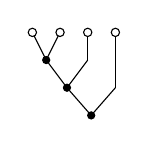
\begin{tikzpicture}[x=1em,y=1em]
		\draw(0,3) -- (0.5,2);
		\draw(1,3) -- (0.5,2);
		\draw(2,3) -- (2,2);
		\draw(3,3) -- (3,2) -- (3,1);
		\draw(0.5,2) -- (1.25,1);
		\draw(2,2) -- (1.25,1);
		\draw(1.25,1) -- (2.125, 0);
		\draw(3,1) -- (2.125, 0);
		\draw[color=black, fill=white](0,3) circle(0.15);
		\draw[color=black, fill=white](1,3) circle(0.15);
		\draw[color=black, fill=white](2,3) circle(0.15);
		\draw[color=black, fill=white](3,3) circle(0.15);
		\fill(2.125,0) circle(0.15);
		\fill (1.25,1) circle(0.15);
		\fill (0.5,2) circle(0.15);
	\end{tikzpicture}
\end{center}
Labelled trees in $\pi_4^{-1}(\{t_7\})$ consists of the following two levelled trees:
\begin{center}
	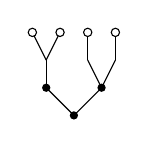
\begin{tikzpicture}[x=1em,y=1em]
		\draw(0,3) -- (0.5,2);
		\draw(1,3) -- (0.5,2);
		\draw(2,3) -- (2,2);
		\draw(3,3) -- (3,2);
		\draw(2,2) -- (2.5,1);
		\draw(3,2) -- (2.5,1);
		\draw(0.5,2) -- (0.5,1);
		\draw(0.5,1) -- (1.5,0);
		\draw(2.5,1) -- (1.5,0);
		\draw[color=black, fill=white](0,3) circle(0.15);
		\draw[color=black, fill=white](1,3) circle(0.15);
		\draw[color=black, fill=white](2,3) circle(0.15);
		\draw[color=black, fill=white](3,3) circle(0.15);
		\fill(1.5,0) circle(0.15);
		\fill (2.5,1) circle(0.15);
		\fill (0.5,1) circle(0.15);
	\end{tikzpicture}
	\hspace{2em}
	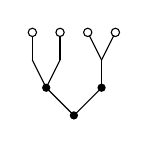
\begin{tikzpicture}[x=1em,y=1em]
		\draw(0,3) -- (0,2);
		\draw(1,3) -- (1,2);
		\draw(2,3) -- (2.5,2);
		\draw(3,3) -- (2.5,2);
		\draw(0,2) -- (0.5,1);
		\draw(1,2) -- (0.5,1);
		\draw(2.5,2) -- (2.5,1);
		\draw(0.5,1) -- (1.5,0);
		\draw(2.5,1) -- (1.5,0);
		\draw[color=black, fill=white](0,3) circle(0.15);
		\draw[color=black, fill=white](1,3) circle(0.15);
		\draw[color=black, fill=white](2,3) circle(0.15);
		\draw[color=black, fill=white](3,3) circle(0.15);
		\fill(1.5,0) circle(0.15);
		\fill (0.5,1) circle(0.15);
		\fill (2.5,1) circle(0.15);
	\end{tikzpicture}
\end{center}

\end{exam}
We want to code \Schw{} trees as levelled Schroeder trees. For this purpose, we need to make a choice of a representative levelled \Schw{} tree of each \Schw{} tree.  

\subsubsection{Our point of view on \Schw{} trees}
\begin{defi}[Initial chains] \label{def:init_chain}
	Let $\mathcal{P}=(P,\leq)$ be a lattice with a minimum and a maximum element.
	Let $C$ be a chain in this poset, we say it is \emph{initial} if $\min(\mathcal{P})$ and $\max(\mathcal{P})$ are in the chain $C$.
\end{defi}
\begin{defi}
	Let $n\in\NN\setminus \{0\}$.
	We define $\IC(\nn)$ the set of strictly increasing \emph{initial chain} of the poset $(\mathcal{P}(\IEM{1}{n}),\subseteq)$. 
\end{defi}
\begin{exam}
	For instance, in the poset $(\mathcal{P}(\IEM{1}{4}),\subseteq)$, we have the following elements of $\IC(4)$:
	\begin{align*}
		\emptyset \subseteq \{1,2,3,4\}, &&
		\emptyset \subseteq \{1,2,3\} \subseteq \{1,2,3,4\}.
	\end{align*}
%	\begin{gather*}
%		\{1\}\{2\}\{3\}\{4\}\leqslant_{\pi} \{1,2,3,4\}, \\
%		\{1\}\{2\}\{3\}\{4\}\leqslant_{\pi} \{1,2,3\}\{4\} \leqslant_{\pi} \{1,2,3,4\}.
%	\end{gather*}
\end{exam}

%\begin{figure}[h]
%	\centering
%	\caption{The $\mathcal{P}(\IEM{1}{4})$ poset with labels on edges}
%	\label{fig:labelled_IP4}
%	\begin{tikzpicture}[rotate =180 ]
%		%Noeud du diagramme
%		\node (P0) at (0,0) {$\{1,2,3,4\}$};
%		\node (P11) at (-2,1) {$\{1,2,3\}\{4\}$};
%		\node (P12) at (0,1) {$\{1,2\}\{3,4\}$};
%		\node (P13) at (2,1) {$\{1\}\{2,3,4\}$};
%		\node(P21) at (-2,2) {$\{1,2\}\{3\}\{4\}$};
%		\node(P22) at (0,2) {$\{1\}\{2,3\}\{4\}$};
%		\node(P23) at (2,2) {$\{1\}\{2\}\{3,4\}$};
%		\node(P31) at (0,3) {$\{1\}\{2\}\{3\}\{4\}$};
%		%Arêtes du poset
%		\draw (P0) -- (P11);
%		\draw (P0) -- (P12);
%		\draw (P0) -- (P13);
%		\draw (P11) -- (P21);
%		\draw (P11) -- (P22);
%		\draw (P12) -- (P21);
%		\draw (P12) -- (P23);
%		\draw (P13) -- (P22);
%		\draw (P13) -- (P23);
%		\draw (P21) -- (P31);
%		\draw (P22) -- (P31);
%		\draw (P23) -- (P31);
%	\end{tikzpicture}
%\end{figure}

But as said previously many levelled \Schw{} trees give a same \Schw{} tree. Hence, for each $n\in \NN$ we want to build a section of $\pi_n$ so that to a \Schw{} tree corresponds a \emph{unique} levelled \Schw{}.

\subsubsection{Our choice of section}

For our use, we introduce the following map:
\begin{prop}\label{prop:trees_to_levels}
	We denote $s:\Sch \rightarrow \Schl$ the unique map such that for any $t\in\Sch$, $s(t)$ is the \emph{unique} levelled \Schw{} tree such that for any internal vertex of $t$, its level is strictly greater than all the internal vertices to its right.
	Then, $s$ is well-defined and this is a section of the map $\pi\coloneqq \displaystyle\bigoplus_{n=0}^{+\infty} \pi_n$.
\end{prop}
\begin{proof}
	To prove $s$ is well-defined, we detail a construction $s(t)$ by induction over the number of leaves of the tree of $t$. Let $t\in\Sch(n)$ with $n\in\NN^*$.
	\begin{description}
		\item[Initialization] for $n=2$, this is obvious as there exists only one representation of $\Y$ as a levelled \Schw{} tree.  
		\item[Heredity] now let us suppose that there exists $n$ such that for any $n'<n, t\in\Sch(n'), s(t)$ is well defined. We consider $t\in\Sch(n+1)$ and let us build $s(t)$. One can see:
		\[
		t=t^{(1)}\vee \dots \vee t^{(k)}
		\]
		where for any $k\geq 2, i\in\IEM{1}{k}, t^{(i)}$ is a \Schw{} tree with at most $n$ leaves.
		Hence, we built $s(t)$ as follows:
		\[
		s(t)=
			\peignegauche{s(t^{(1)})}{s(t^{(2)})}{s(t^{(k)})}
		\]
	\end{description}
	Finally by construction, we have $\pi\circ s=\Id_{\Sch}$ 	
\end{proof}
\begin{exam}
	Consider the tree
	\begin{center}
	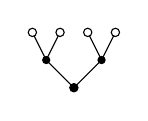
\begin{tikzpicture}[x=1em,y=1em]
		\draw(0,2) -- (0.5,1);
		\draw(1,2) -- (0.5,1);
		\draw(2,2) -- (2.5,1);
		\draw(3,2) -- (2.5,1);
		\draw(0.5,1) -- (1.5,0);
		\draw(2.5,1) -- (1.5,0);
		\draw[color=black, fill=white](0,2) circle(0.15);
		\draw[color=black, fill=white](1,2) circle(0.15);
		\draw[color=black, fill=white](2,2) circle(0.15);
		\draw[color=black, fill=white](3,2) circle(0.15);
		\filldraw[color=black] (1.5,0) circle(0.15);
		\fill (2.5,1) circle(0.15);
		\fill (0.5,1) circle(0.15);
	\end{tikzpicture}
\end{center}
	The only tree satisfying this definition among its two representatives is:
	\begin{center}
		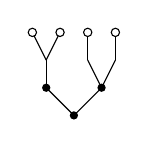
\begin{tikzpicture}[x=1em,y=1em]
			\draw(0,3) -- (0.5,2);
			\draw(1,3) -- (0.5,2);
			\draw(2,3) -- (2,2);
			\draw(3,3) -- (3,2);
			\draw(2,2) -- (2.5,1);
			\draw(3,2) -- (2.5,1);
			\draw(0.5,2) -- (0.5,1);
			\draw(0.5,1) -- (1.5,0);
			\draw(2.5,1) -- (1.5,0);
			\draw[color=black, fill=white](0,3) circle(0.15);
			\draw[color=black, fill=white](1,3) circle(0.15);
			\draw[color=black, fill=white](2,3) circle(0.15);
			\draw[color=black, fill=white](3,3) circle(0.15);
			\fill(1.5,0) circle(0.15);
			\fill (0.5,1) circle(0.15);
			\fill (2.5,1) circle(0.15);
		\end{tikzpicture}
	\end{center}
\end{exam}

\subsubsection{The encoding}

Using the section $s$, we can identify any \Schw{} tree with a finite list of binary words thanks to the map defined below

\begin{defi}
	Let $t$ be a planar tree and let $v\in V(t)$. An \emph{angle} of $t$ on $v$ is a pair $(x,y)\in V(t), x\neq y$ of adjacent vertices to $v$ such that the path from the root to $v$ does not contain $x$ or $y$ and the segment from $x$ to $y$ does not cross the tree.
\end{defi}

\begin{defi}\label{defi:lifetime}
	For any $n\in\NN,$ we introduce a map $\varphi_n: \Schl(n)\rightarrow \IC(\IEM{1}{n})$ defined for any $t\in\Schl(n)$ by the \emph{unique} initial chain describing the lifetime of the angles of $t$ in function of the levels of the tree.
	
	We also define $\Set_n$, the map sending any element of $\IC(\IEM{1}{n})$ onto a list of length $n$ with $0$'s and $1$'s encoding the element of $\mathcal{P}(\IEM{1}{n})$ considered. More precisely, for any ${X\in\mathcal{P}(\IEM{1}{n})}$:
	\[
	\Set_n(X)\coloneq (\mathbbm{1}_X(i))_{i\in\IEM{1}{n}}.
	\]
\end{defi}
\begin{exam}\label{Eg:tree_code}
	For instance, reading sequences from top to bottom:
	\begin{align}
		\raisebox{-0.5\height}{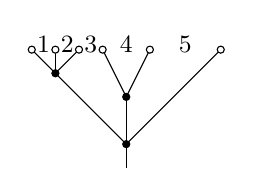
\begin{tikzpicture}[x=0.3cm, y=0.3cm]
				\draw (0,0)--(0,1);
				\draw (0,1)--(-4,5);
				\draw (0,1)--(4,5);
				\draw (0,1)--(0,3);
				\draw (0,3)--(-1,5);
				\draw (0,3)--(1,5);
				\draw (-3,4)--(-2,5);
				\draw (-3,4)--(-3,5);
				% dessin des noeuds
				\filldraw (0,1) circle (0.15);
				\draw[ color=black, fill=white]  (-4,5) circle (0.15);
				\draw[ color=black, fill=white]  (-3,5) circle (0.15);
				\draw[ color=black, fill=white]  (-2,5) circle (0.15);
				\draw[ color=black, fill=white]  (-1,5) circle (0.15);
				\draw[ color=black, fill=white]  (4,5) circle (0.15);
				\draw[ color=black, fill=white]  (1,5) circle (0.15);
				\filldraw (-3,4) circle (0.15);
				\filldraw (0,3) circle (0.15);		
				% Décorations angulaires
				\draw (-3.5, 5.2) node{\small{$1$}};
				\draw (-2.5, 5.2) node{\small{$2$}};
				\draw (-1.5,5.2) node{\small{$3$}};
				\draw (0, 5.2) node{\small{$4$}};
				\draw (2.5, 5.2) node{\small{$5$}};
		\end{tikzpicture}} && \overset{\varphi_5}{\longrightarrow} && \begin{array}{c}
			\IEM{1}{5} \\
			\IEM{3}{5} \\
			\{3\}~\{5\} \\
			\emptyset
		\end{array}
		&& \overset{\Set_5}{\longrightarrow} &&  \begin{array}{ccccc}
			1 & 1 & 1 & 1 & 1 \\
			0 & 0 & 1 & 1 & 1 \\
			0 & 0 & 1 & 0 & 1 \\
			0 & 0 & 0 & 0 & 0
		\end{array} 
		%&& \overset{B}{\longrightarrow} && \begin{array}{c}
%			31 \\ 28 \\ 20 \\ 0
%		\end{array}
	\end{align}
\end{exam}

\begin{Not}
	We will call the \emph{code map}, denoted $\Code$, the map $\Set\circ\varphi\circ s:\Sch\to \IC$ where:
	\[
	\IC \coloneqq \bigoplus_{n=0}^{+\infty} \IC(\IEM{1}{n}).
	\]
\end{Not}
Thanks to this result we can now encode one \Schw{} tree as a list of integers/sequences over $\{0,1\}$ into a computer. Now, we can look at the action of quasi-shuffles on our encoding of trees for an easy computation in the free tridendriform algebra with one generator.

%\PCt{Je mets une partie pour décrire l'image des $\varphi_n$ que l'on ne conservera peut-être pas.}
%
%\subsubsection{Description of the image of \Schw{} trees}
%
%We can notice that the image of $\varphi\circ s$, where $\varphi=\displaystyle\bigoplus_{n=0}^{+\infty} \varphi_n$, is strictly included inside $\displaystyle \bigoplus_{n=0}^{+\infty} \IC(\IEM{1}{n})$. We give here a description of the image of $\varphi$. For this purpose we need to introduce some definitions:
%\begin{defi}
%	Let $n\in\NN$ and $x\in\mathcal{P}(\IEM{1}{n})$. An \emph{interval} in $x$ is a subset of $x$ of the shape $\IEM{i}{j}$ with $i<j.$
%	We will denote $\Con(x)$ the set of maximal intervals in $x$.
%\end{defi}
%With this connectivity concept, we have:
%\[
%x=\bigcup_{c\in\Con(x)} c.
%\]
%\begin{Rq}
%	Let $n\in\NN$ et $x\in\mathcal{P}(\IEM{1}{n})$.
%	Note that $\Con(x)$ has a total order induced by the order of the minimum of each block. More precisely, for $(c_1,c_2)\in\Con(x)$:
%	\[
%	c_1<c_2 \iff \min(c_1)<\min(c_2).
%	\]
%\end{Rq}
%\begin{defi}
%	Let $n\in\NN$ and consider $C\in\IC(\IEM{1}{n})$. Let $x\in C$ which is not an extrema of $C$. We denote by $\prev{x}$ the previous element in the chain $C$.  We denote by $\suiv{x}$ the next element in the chain $C$. 
%\end{defi}
% 
% \begin{prop}
% 	We have $C\in\ima(\varphi\circ s)$ if and only if:
% 	\[
% 	\forall x\in C\setminus\{\max(C)\}, \forall c\in\Con(x), \forall c'\in \Con(x), c'>c \implies c'\in \suiv{x}.
% 	\]
% \end{prop}
%\begin{proof}
%	Todo
%\end{proof}
%\PCt{Est-ce qu'on parle des suites croissantes pour le poids de Hamming ?} 

\subsection{The tridendriform structure on $\ima(\Code)$}

One usual operation we can perform on words is the concatenation. In our particular case, the tridendriform operations over $\IC{}$ are more complicated. In fact, we could multiply two initial chains with partition set of different lengths.
\begin{Rq}
	For now on, for any $n\in\NN$ we will no longer distinguish elements of $\IC(\IEM{1}{n})$ and its image by the map $\Set$. We also allow ourselves to mix the notations.
\end{Rq}

\subsubsection{Preliminary definitions}

In order to describe properly to the computer what we want to do, we have to identify elements encoding the comb representation of the tree associated to it. 

%TODO Notation setminus pour les suites à définir
\begin{defi}[forest code]\label{defi:forest_codes}
	Let $n\in\NN$. Let $C'\in\IC(\IEM{1}{n})$ %be an initial chain of the set $\IEM{1}{n}$
	 and put $C=C'\setminus \max(C')$.
	Any $C$ satisfying this property will be called a \emph{forest code}. 
	The \emph{forest} associated to a forest code is the ordered concatenation of trees we get deleting the root of the tree encoded by $C'$. 
\end{defi}
\begin{Rq}
	The forest code associated to the empty chain, denoted $\varepsilon$, is $\unitree$. 
	Note that if $C$ is a forest code that is not an initial chain, then there exists a unique forest $F$ such that $\Code(T)=C'$ where $T$ is the grafting of all the element of the forest $F$ in this order to a common root. Hence, we extend the definition of the map $\Code$ to forests codes in such a way that $\Code(F)=C.$ 
\end{Rq}
\begin{exam}
	For instance, the forest code $\Code\left(\balaisd~\Y~\unitree\right)$ is:
	\[
	\begin{array}{ccccc}
	1 & 1 & 1 & 1 & 1 \\
	1 & 0 & 1 & 1 & 1 \\
	0 & 0 & 1 & 1 & 1 \\
	0 & 0 & 1 & 0 & 1
	\end{array}
	\] 
	Note that $\Code\left(\unitree~\unitree~\unitree\right)=1~1.$
\end{exam}

\begin{defi}[left comb decomposition]
	Let $n\in\NN$ and $C\in\IC(\IEM{1}{n})$.
	Its \emph{left comb decomposition}, denoted \LCD{C}, is obtained inductively the following way:
	\begin{gather*}
	\LCD{\varepsilon}=\varepsilon \\
	\LCD{C}=( \LCD{C_1}, F_1),
	\end{gather*}
	where in the induction we assumed $A\times (B \times C)\approx (A\times B) \times C$, and $F_1$ and $C_1$ satisfy the following block equality:
	\[
	C=\begin{tblr}{vlines, colspec={ccc}, cell{1}{1}={r=3}{c}, cell{1}{3}={r=3}{c}, column{2}={bg=red!25}
}
	\tilde{C_1} & 1  & \tilde{F_1} \\
	 C_1 & \vdots & F_1 \\
	 C_1 & 1  & F_1 \\
	 0\cdots 0 &0  & 0 \cdots 0
	\end{tblr} \text{ if it is a tree code or }
	C=\begin{tblr}{vlines, colspec={ccc}, cell{1}{1}={r=3}{c}, cell{1}{3}={r=3}{c}, column{2}={bg=red!25}
	}
	\tilde{C_1} & 1  & \tilde{F_1} \\
	C_1 & \vdots & F_1 \\
	C_1 & 1  & F_1 
	\end{tblr} \text{ if it is a forest code.}
	\]
	such that $F_1$ and $C_1$ are respectively $\tilde{F_1}$ and $\tilde{C_1}$ keeping only once any instance of a integer sequence. Moreover, the red line spotted is the \emph{leftmost} column with this property in $C$. 
\end{defi}
\begin{exam}
	We will start from a tree, consider its code, we apply the decomposition detailed above and compare  the left comb decomposition of the tree with the forest associated to the sequence of the forest code.
	\[
	s=\raisebox{-0.3\height}{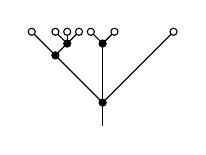
\begin{tikzpicture}[x=0.3cm, y=0.3cm]
	%structure de l'arbre
	\draw (0,0) -- (0,1);
	\draw (0,1) -- (-3,4);
	\draw (0,1) -- (3,4);
	\draw (0,1) -- (0,3.5);
	\draw (0,3.5) -- (0.5,4);
	\draw (0,3.5) -- (-0.5,4);
	\draw (0,3.5) -- (0.5,4);
	\draw (-2,3) -- (-1,4);
	\draw (-1.5,3.5) -- (-1.5,4);
	\draw (-1.5,3.5) -- (-2,4);	
	%les cercles
	\filldraw[color=black,fill=white] (-3,4) circle (0.15);
	\filldraw[color=black,fill=white] (-2,4) circle (0.15);
	\filldraw[color=black,fill=white] (-1.5,4) circle (0.15);
	\filldraw[color=black,fill=white] (-1,4) circle (0.15);
	\filldraw[color=black,fill=white] (-0.5,4) circle (0.15);
	\filldraw[color=black,fill=white] (0.5,4) circle (0.15);
	\filldraw[color=black,fill=white] (3,4) circle (0.15);	
	\filldraw (0,1) circle (0.15);
	\filldraw (-2,3) circle (0.15);
	\filldraw (-1.5,3.5) circle (0.15);
	\filldraw (0,3.5) circle (0.15);
	\end{tikzpicture}} \longrightarrow \begin{tblr}{colspec={cccccc}, column{4}={bg=blue!25}}
	1 & 1 & 1 & 1 & 1 & 1 \\
	1 & 0 & 0 & 1 & 1 & 1 \\
	0 & 0 & 0 & 1 & 1 & 1 \\
	0 & 0 & 0 & 1 & 0 & 1 \\
	0 & 0 & 0 & 0 & 0 & 0
	\end{tblr} = \Code(s) \eqqcolon S.
	\] 
	Hence:
	\begin{align*}
		\LCD{S}&=\left(\LCD{\begin{tblr}{colspec={ccc}, column{1}={bg=blue!25}}
		1 & 1 & 1 \\
		1 & 0 & 0 \\
		0 & 0 & 0
		\end{tblr}}, \begin{tblr}{colspec={cc}}
			1 & 1 \\
			0 & 1
			\end{tblr}\right) \\
		&=\left(\varepsilon, \begin{tblr}{colspec={cc}}
		1 & 1 \\
		0 & 0
		\end{tblr}, \begin{tblr}{colspec={cc}}
		1 & 1 \\
		0 & 1
		\end{tblr}\right).
	\end{align*}
	Associating to it the $3$-uplet of the forests code by inverting $\Code$ and applying it component-wise, we have:
	\[
	\left( \unitree, \balais{}, \Y{}~\unitree\right).
	\]
	%TODO Il faut enlever le premier vide à gauche
	We have recovered the left comb decomposition of $s$ after forgetting the leftmost $\unitree$.
\end{exam}

\begin{defi}[right comb decomposition]
		Let $n\in\NN$ and $C\in\IC(\IEM{1}{n})$.
		Its \emph{right comb decomposition}, denoted \RCD{C}, is obtained inductively the following way:
		\begin{gather*}
		\RCD{\varepsilon}=\varepsilon \\
		\RCD{C}=( F_1, \RCD{C_1} ),
		\end{gather*}
		where in the induction we assumed $A\times (B \times C)\approx (A\times B) \times C$, and $F_1$ and $C_1$ satisfy the following block equality:
		\[
		C=\begin{tblr}{vlines, colspec={ccc}, cell{1}{1}={r=3}{c}, cell{1}{3}={r=3}{c}, column{2}={bg=red!25}
		}
		\tilde{F_1} & 1  & \tilde{C_1} \\
		F_1 & \vdots & C_1 \\
		F_1 & 1  & C_1 \\
		0\cdots 0 &0  & 0 \cdots 0
		\end{tblr} \text{ if it is a tree code or }C=\begin{tblr}{vlines, colspec={ccc}, cell{1}{1}={r=3}{c}, cell{1}{3}={r=3}{c}, column{2}={bg=red!25}
		}
		\tilde{F_1} & 1  & \tilde{C_1} \\
		F_1 & \vdots & C_1 \\
		F_1 & 1  & C_1 
		\end{tblr} \text{ if it is a forest code.}
		\]
		such that $F_1$ and $C_1$ are respectively $\tilde{F_1}$ and $\tilde{C_1}$ keeping only once any instance of a integer sequence. Moreover, the red line spotted is the \emph{rightmost} column in $C$ ending with a $1$ or with a unique $0$ if the last line is full of zeros. 
\end{defi}
\begin{exam}
		We will start from a tree, consider its code, then apply the decomposition detailed above and compare  the right comb decomposition of the tree with the forest associated to the sequence of forest code.
	\[
	t=\raisebox{-0.3\height}{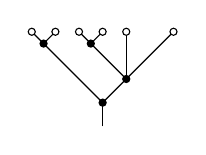
\begin{tikzpicture}[x=0.3cm, y=0.3cm]
	%structure de l'arbre
	\draw (0,0) -- (0,1);
	\draw (0,1) -- (3,4);
	\draw (0,1) -- (-3,4);
	\draw (-2.5,3.5) -- (-2,4);
	\draw (1,2) -- (-1,4);
	\draw (1,2) -- (1,4);
	\draw (-0.5,3.5) -- (0,4);	
	%les cercles
	\filldraw[color=black,fill=white] (3,4) circle (0.15);
	\filldraw[color=black,fill=white] (1,4) circle (0.15);
	\filldraw[color=black,fill=white] (0,4) circle (0.15);
	\filldraw[color=black,fill=white] (-1,4) circle (0.15);
	\filldraw[color=black,fill=white] (-2,4) circle (0.15);
	\filldraw[color=black,fill=white] (-3,4) circle (0.15);
	\filldraw (0,1) circle (0.15);
	\filldraw (-2.5,3.5) circle (0.15);
	\filldraw (1,2) circle (0.15);
	\filldraw (-0.5,3.5) circle (0.15);
	\end{tikzpicture}} \longrightarrow \begin{tblr}{colspec={ccccc}, column{2}={bg=blue!25}}
	1 & 1 & 1 & 1 & 1 \\
	0 & 1 & 1 & 1 & 1 \\
	0 & 1 & 0 & 1 & 1 \\
	0 & 1 & 0 & 0 & 0 \\
	0 & 0 & 0 & 0 & 0
	\end{tblr} =\Code(t)\eqqcolon T
	\] 
	Hence:
	\begin{align*}
		\RCD{T}&=\left(\begin{tblr}{colspec={c}}
		1  \\
		0
		\end{tblr}, \RCD{\begin{tblr}{colspec={ccc}, column{3}={bg=blue!25}}
			1 & 1 & 1 \\
			0 & 1 & 1
			\end{tblr}}\right) \\
		&=\left(\begin{tblr}{colspec={c}}
		1  \\
		0
		\end{tblr}, \begin{tblr}{colspec={cc}}
			1 & 1  \\
			0 & 1 
			\end{tblr},\varepsilon\right)
	\end{align*}
	Associating to it the $3$-uplet of the forests code, we have:
	\[
	\left( \Y, \Y~\unitree, \unitree\right).
	\]
	We have recovered the comb decomposition of $t$ after forgetting the rightmost $\unitree$.
\end{exam}

\begin{defi}
	For any \Schw{} tree $t$, we define respectively the \emph{right tree length} and the \emph{left tree length} by:
	\[
	\RTL(t)\coloneqq|\RCD{t}|-1 \text{ and }\LTL(t)\coloneqq |\LCD{t}|-1.
	\]
\end{defi}

Now, we have an analogous of the comb decomposition for our sequences. We can now describe the action of a quasi-shuffle on these objects.

\subsubsection{The tridendriform structure for initial chains}

By analogy with \Schw{} trees, we put:

\begin{defi}\label{defi:quasishuffle_code}
	Let $T\in\IC(\IEM{1}{n})$ and $S\in\IC(\IEM{1}{m})$. Let us denote $k=\RTL(T)$ and $l=\LTL(S)$. Consider $\sigma\in\batc(k,l)$ which has for image $\IEM{1}{r}$. We denote by $\sigma(T,S)$ the element of $\IC(\IEM{1}{m+n})$ defined by:
	\begin{enumerate}
		\item on the first $m$ integers, copy all the $k$ forests codes of $\RCD{T}$ (excepted to the rightmost one $\unitree$) separated by a column of ones on their right;  
		\item for $h$ from $r$ to $1$ with a $-1$ step: %Je ne sais pas trop comment tourner ça !
		\begin{description} % TODO à réécrire en mettant de bonnes notations pour RCD et LCD
			\item[Case 1] if $\sigma^{-1}(\{h\})=\{i\}, i\in\IEM{1}{k}$, write $0$'s below the code of $F_i$ and on its adjacent right column.
			\item[Case 2] if $\sigma^{-1}(\{h\})=\{j\}, j\in\IEM{k+1}{k+l}$, include the code of $F_j$ at its appropriate place shifted by $n$ with a ones column on its left write $0$'s below the code of $F_j$ and on its adjacent left column. Write $0$'s below the code of $F_j$ and on its adjacent left column.
			\item[Case 3] if $\sigma^{-1}(\{h\})=\{i,j\}, (i,j)\in\IEM{1}{k}\times\IEM{k+1}{k+l}$, include the code of $F_j$ at its appropriate place shifted by $n$ with a ones column on its left. Write $0$'s below the code of $F_j$ and on its adjacent left column. Then, write $0$'s below the code of $F_j$ and on its adjacent left column \emph{and} below the code of $F_i$ and on its adjacent right column.
		\end{description}
		The element obtained from this operation is denoted $\sigma(T,S)$.
	\end{enumerate} 
\end{defi}
\begin{Rq}
	For this operation, one should remind the ending positions of each forest code.
\end{Rq}

\begin{exam}
		Consider the $(2,2)$-quasi-shuffle $\sigma=(1,3,2,3)$. Let us take 
	$t=$	\raisebox{-0.3\height}{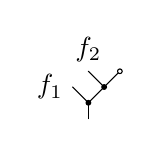
\begin{tikzpicture}[line cap=round,line join=round,>=triangle 45,x=0.2cm,y=0.2cm]
		% Etage 1
		\draw (0,0)--(0,1);
		%Etage 2
		\draw (0,1)--(-1,2) node[left]{$f_1$};
		% Etage 3
		\draw (0,1)--(2,3);
		\draw (1,2)--(0,3) node[left,above]{$f_2$};
		%marquages des sommets
		\filldraw (0,1) circle (0.15);
		\filldraw (1,2) circle (0.15);
		\draw[color=black, fill=white] (2,3) circle (0.15);
		\end{tikzpicture}} and $s=\raisebox{-0.3\height}{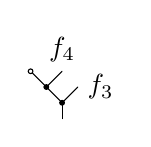
\begin{tikzpicture}[line cap=round,line join=round,>=triangle 45,x=0.2cm,y=0.2cm]
		% Etage 1
		\draw (0,0)--(0,1);
		%Etage 2
		\draw (0,1)--(1,2) node[right]{$f_{3}$};
		% Etage 3
		\draw (0,1)--(-2,3);
		\draw (-1,2)--(0,3) node[right,above]{$f_{4}$};
		%marquages des sommets
		\filldraw (0,1) circle (0.15);
		\filldraw (-1,2) circle (0.15);
		\draw[color=black, fill=white] (-2,3) circle (0.15);
		\end{tikzpicture}}$.
	Then $\sigma(t,s)=$\raisebox{-0.5\height}{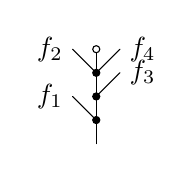
\begin{tikzpicture}[line cap=round,line join=round,>=triangle 45,x=0.3cm,y=0.3cm]
		\draw (0,0)--(0,4);
		%Noeud 1
		\draw (0,1)--(-1,2) node[left]{$f_1$};
		%Noeud 2
		\draw (0,2)--(1,3) node[right]{$f_3$};
		%Noeud 3
		\draw (0,3)--(-1,4) node[left]{$f_2$};
		\draw (0,3)--(1,4) node[right]{$f_4$};
		%marquage des noeuds
		\filldraw (0,1) circle (0.15);
		\filldraw (0,2) circle (0.15);
		\filldraw (0,3) circle (0.15);
		\draw[color=black, fill=white] (0,4) circle (0.15);
		\end{tikzpicture}}.
	Then, let us denote for all $i\in\IEM{1}{4}, \Code(f_i)=F_i$.
	Hence, the code associated to $t$ and $s$ respectively denoted $T$ and $S$ are of the shape:
	\[
	T=\begin{tblr}{colspec={cccccc},
	cell{2}{1}={r=3,c=2}{c},
	cell{5}{4}={r=3,c=2}{c}
	}
	1 & \cdots & 1 & 1 & \cdots &  1 \\
	F_1 & F_1 & 1 & 1  & \cdots & 1 \\
	F_1  & F_1 & \vdots &1   & \cdots & 1 \\
	F_1 & F_1  & 1 & 1 & \cdots & 1  \\
	\vdots & \vdots & 1 & F_2 &  &  1 \\
	\vdots & \vdots & 1 & F_2 & & \vdots\\
	\vdots & \vdots & 1 & F_2 &  & 1 \\
	\vdots & \vdots & 1 & 0 & \cdots & 0 \\
	0 & \cdots & 0 & 0 & \cdots & 0
	\end{tblr} \text{ and }
	S=\begin{tblr}{colspec={cccccc},
		 cell{2}{2}={r=3,c=2}{c},
		cell{6}{5}={r=3,c=2}{c}
	}
	   1 & \cdots & 1 & 1 & \cdots &  1 \\
	   1 &  F_4 & F_4 &1  & \cdots & 1 \\
	   \vdots & F_4  & F_4 &1   & \cdots & 1 \\
	   1 & F_4 & F_4  & 1 & \cdots & 1  \\
	   0 & \cdots & 0 & 1 & \cdots & 1  \\
	   0 & \cdots & 0 &1 & F_3 &  \\
	   0 & \cdots & 0 & \vdots  & F_3 & \\
	   0 & \cdots & 0 & 1 & F_3 &  \\
	   0 & \cdots & 0 & 0 & \cdots & 0 
	\end{tblr}
	\]
	Then, $\sigma(T,S)$ is the code of the tree $\sigma(t,s)$ given by:
	\[
	\begin{tblr}{colspec={cccccccccccc},
			cell{2}{1}={r=3,c=2}{c},
			cell{5}{4}={r=3,c=2}{c},
			cell{8}{8}={r=3,c=2}{c},
			cell{12}{11}={r=3,c=2}{c},
			row{11}={bg=blue!25},
			row{15}={bg=red!25},
			row{16}={bg=yellow!50}
		}
		1 & \cdots & 1 & \cdots & \cdots & \cdots & \cdots & \cdots & \cdots & \cdots & \cdots & 1 \\
		F_1 & F_1 & 1 	   & \cdots & \cdots & \cdots & \cdots & \cdots & \cdots & \cdots & \cdots & 1 \\
		F_1 & F_1 & \vdots & \cdots & \cdots & \cdots & \cdots & \cdots & \cdots & \cdots & \cdots & \vdots \\
		F_1 & F_1 &	   	 1 & 1 		& \cdots & 	1	  & 	1  & \cdots & \cdots & \cdots & \cdots  & 1 \\
		\vdots & \vdots & \vdots & F_2 & F_2 & \vdots & \vdots & \cdots & \cdots & \cdots & \cdots  & \vdots \\
		\vdots & \vdots & \vdots & F_2 & F_2 & 1 & 1 & \cdots & \cdots & \cdots & \cdots  & 1 \\
		\vdots & \vdots & 1		 & F_2 & F_2 & 1 & 1 & \cdots & \cdots & 1  & \cdots & 1 \\
		\vdots & \vdots & 1		& \vdots & \vdots & 1 	   & 1 		& F_4  & F_4 & \vdots & \cdots  & \vdots \\
		\vdots & \vdots & 1		& \vdots & \vdots & \vdots & \vdots & F_4  & F_4 & \vdots & \cdots  & \vdots \\
		\vdots & \vdots & 1		& \vdots & \vdots & 1 	   & 1	    & F_4  & F_4 & 	1    & \cdots & 1 \\
		\vdots & \vdots & 1		& 0      & \cdots & 0 	   & 0	    &\cdots& 0   & 1 & \cdots & 1 \\
		\vdots & \vdots & 1		& 0      & \cdots & 0 	   & 0	    &\cdots& 0	 	 & 1      & F_3  & F_3 \\
		\vdots & \vdots & 1		& 0      & \cdots & 0 	   & 0	    &\cdots& \vdots  & \vdots & F_3  & F_3 \\
		\vdots & \vdots & 1		& 0      & \cdots & 0 	   & 0	    &\cdots& 	0 	 &	  1   & F_3  & F_3 \\
		\vdots & \vdots & 1		& 0      & \cdots & 0 	   & 0	    &\cdots& \cdots  &	  0   &\cdots& 0 \\
		0	   & \cdots & \cdots& \cdots & \cdots & 0      & 0	    &\cdots& \cdots  &	  0   &\cdots& 0 
	\end{tblr}
	\]
\end{exam}

With this definition, we are now able to define three operators in $\ima(\Code)$

\begin{defi}\label{defi:operations_codes}
	Let $T$ and $S$ be two elements in $\ima(\Code)$ such that ${k=|\RTL(T)|}$ and ${l=|\LTL(S)|}$. We define:
	\begin{align*}
		T \prec S= \sum_{\substack{\sigma\in\batc(k,l) \\ \sigma^{-1}(\{1\})=\{1\}}} \sigma(T,S), &&
		T \succ S= \sum_{\substack{\sigma\in\batc(k,l) \\ \sigma^{-1}(\{1\})=\{1\}}} \sigma(T,S), \\
		T \cdot S= \sum_{\substack{\sigma\in\batc(k,l) \\ \sigma^{-1}(\{1\})=\{1,k+1\}}} \sigma(T,S). \\
	\end{align*}
\end{defi}

In the sequel, we show that this structure is a tridendriform structure on $\ima(\Code)$ showing it is isomorphic to the free tridendriform algebra of \Schw{} trees. Hence it gives us a mathematical background to implement programs in section~\ref{sec:coding}.

\begin{thm} 
	Let $t,s$ be two \Schw{} trees with shapes given in equation~\eqref{eq:tree_combs}. Hence, $k$ is the right comb length of $t$ and $l$ the left comb length of $s$. Let $\sigma\in\batc(k,l)$. Then:
	\[
	\Code(\sigma(t,s))= \sigma(\Code(t),\Code(s)).
	\]
\end{thm}
\begin{proof}
In order to prove this theorem, we will proceed by induction over the sum of $k$ and $l$. If $l=0$ or $k=0$, this means that $s=\unitree$ or $t=\unitree$. We initialize the induction $0,1$ and $2$.
\begin{description}
	\item[Initialization] if $\max(k,l)=1$ and $k+l=1$, then the identity shuffle is acting on this pair of tree and one of them is $\unitree$. By definition~\ref{defi:quasishuffle_code}, we get back the tree code of the non-unit element.
	Otherwise, if $k+l=2$ and $k,l\neq 0$ hence $\sigma=(1,1)$, then:
	\[
	t=\raisebox{-0.3\height}{\begin{tikzpicture}[x=0.25cm,y=0.25cm]
		\draw (0,0) -- (0,1);
		\draw (0,1) -- (1,2);
		\draw (0,1) -- (-1,2);
		\draw (-1,2) node[left] {$f_1$};
	\end{tikzpicture}}, 
	s=\raisebox{-0.3\height}{\begin{tikzpicture}[x=0.25cm,y=0.25cm]
		\draw (0,0) -- (0,1);
		\draw (0,1) -- (1,2);
		\draw (0,1) -- (-1,2);
		\draw (1,2) node[right] {$f_2$};
	\end{tikzpicture}} \text{ and } \sigma(t,s)=\raisebox{-0.3\height}{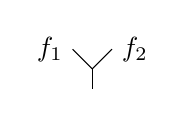
\begin{tikzpicture}[x=0.25cm,y=0.25cm]
	\draw (0,0) -- (0,1);
	\draw (0,1) -- (1,2);
	\draw (0,1) -- (-1,2);
	\draw (1,2) node[right] {$f_2$};
	\draw (-1,2) node[left] {$f_1$};
	\end{tikzpicture}}
	\]
	Denoting $\Code(f_1)=F_1$ and $\Code(f_2)=F_2$, their respective codes are:
	\[
	T=\begin{tblr}{colspec={ccc},
			cell{2}{1}={r=3,c=2}{c}
		}
		1 & \cdots & 1 \\
		F_1 & F_1 & 1 \\
		F_1 & F_1 & \vdots \\
		F_1 & F_1 & 1 \\
		0 & \cdots & 0 \\
	\end{tblr}, S=\begin{tblr}{colspec={ccc},
		cell{2}{2}={r=3,c=2}{c}
	}
	1 & \cdots & 1 \\
	1 & F_2 & F_2 \\
	1 & F_2 & F_2 \\
	1 & F_2 & F_2 \\
	0 & \cdots & 0 \\
	\end{tblr} \text{ and } \sigma(T,S)=\begin{tblr}{colspec={cccccccc},
		cell{2}{1}={r=3,c=3}{c},
		cell{5}{6}={r=3,c=3}{c},
	}
	1 & \cdots & 1 & 1 & 1 & 1 & \cdots & 1\\
	F_1 & F_1 & F_1 & 1 & 1 & 1 & \cdots & 1 \\
	F_1 & F_1 & 1 & \vdots & \vdots & \vdots & \vdots & \vdots \\
	F_1 & F_1 & 1 & 1 & 1 & 1 & \cdots & 1 \\
	0 & \cdots & 0 & 1 & 1 & F_2 & F_2 & F_2 \\
	0 & \cdots & 0 & \vdots & \vdots & F_2 & F_2 & F_2\\
	0 & \cdots & 0 & 1 & 1 & F_2 & F_2 & F_2\\
	0 & \cdots & 0 & 0 & 0 & 0 & \cdots & 0\\
	\end{tblr}
	\]
	Note that the code of $\sigma(T,S)$ has for associated tree $\sigma(t,s)$. If $k=0$ or $l=0$, then the result is obvious.
	\item[Heredity] Suppose that there exists $r \geq 1\in\NN^*$ such that for all couple $(k,l)$ with $k+l\leq r$, we have for any $t,s$ whose tree length are respectively $k$ and $l$:
	\[
	\sigma(\Code(t),\Code(s))=\Code(\sigma(t,s)).
	\]
	Let us prove that this property is true for the next rank. Let $t,s$ be two trees with right comb length $k$ and left comb length $l$, let $\sigma\in\bat(k,l)$ such that $k+l=r+1$. Note that if $k=0$ or $l=0$, the result is obvious by definition~\ref{defi:operations_codes}. There are three possible cases left, in those cases, we use the notations of the proof of lemma~\ref{lem:Indution_batc}:
	\begin{description} 
		\item[First case] $\sigma^{-1}(\{1\})=\{1\}$:
		Then:
		\begin{align*}
			\Code(\sigma(t,s))&=\Code\left(\raisebox{-0.3\height}{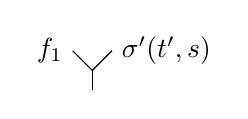
\begin{tikzpicture}[x=0.25cm,y=0.25cm]
				\draw (0,0) -- (0,1);
				\draw (0,1) -- (-1,2);
				\draw (0,1) -- (1,2);
				\draw (-1,2) node[left] {$f_1$};
				\draw (1,2) node[right] {$\sigma'(t',s)$};
			\end{tikzpicture}}\right)\text{ where } t'=\raisebox{-0.3\height}{\begin{tikzpicture}[x=0.25cm,y=0.25cm]
			\draw (0,0) -- (0,1);
			\draw (0,1) -- (-1,2);
			\draw (0,1) -- (1,2);
			\draw (-1,2) node[left] {$f_1$};
			\draw (1,2) node[right] {$t'$};
		\end{tikzpicture}}, \\
		&=\begin{tblr}{colspec={cccccc},
				cell{2}{1}={r=3,c=2}{c},
				cell{5}{4}={r=3,c=3}{c}
			}
			1 & \cdots & 1 & 1 & \cdots & 1 \\
			F_1 & F_1 & 1 & 1 & \cdots & 1 \\
			F_1 & F_1 & \vdots & 1 & \cdots & 1 \\
			F_1 & F_1 & 1 & 1 & \cdots & 1 \\
			\vdots & \vdots & 1 	   &  \Code(\sigma'(t',s)) & \sigma(t',s) & \sigma(t',s)  \\
			\vdots & \vdots & \vdots   &  \sigma(t',s) & \sigma(t',s) & \sigma(t',s)  \\
			\vdots & \vdots & 1	       &  \sigma(t',s) & \sigma(t',s) & \sigma(t',s) \\
			0 & \cdots & 0 & 0 & \cdots & 0
		\end{tblr}
		\end{align*}
		Applying the induction hypothesis because $\RTL(t')+\LTL(s)\leq r$, we have:
		\begin{align*}
			\Code(\sigma(t,s))&=\begin{tblr}{colspec={cccccc},
					cell{2}{1}={r=3,c=2}{c},
					cell{5}{4}={r=3,c=3}{c}
				}
				1 & \cdots & 1 & 1 & \cdots & 1 \\
				F_1 & F_1 & 1 & 1 & \cdots & 1 \\
				F_1 & F_1 & \vdots & 1 & \cdots & 1 \\
				F_1 & F_1 & 1 & 1 & \cdots & 1 \\
				\vdots & \vdots & 1 	   &  \sigma'(\Code(t'),\Code(s)) & \sigma(t',s) & \sigma(t',s)  \\
				\vdots & \vdots & \vdots   &  \sigma(t',s) & \sigma(t',s) & \sigma(t',s)  \\
				\vdots & \vdots & 1	       &  \sigma(t',s) & \sigma(t',s) & \sigma(t',s) \\
				0 & \cdots & 0 & 0 & \cdots & 0
			\end{tblr} \\
			&= \sigma(\Code(t), \Code(s)),
		\end{align*}
		by definition of the action of $\sigma$ over a pair of forests codes.
	\item[Second case] $\sigma^{-1}(\{1\})=\{k+1\}$ %, we denote $\sigma'$ the unique element of $\batc(k,l-1)$ such that:
%		\[
%		\forall n\in\IEM{1}{k+l}, \sigma(n)=\begin{cases}
%			k+1 &\text{ if } n=k+1, \\
%			\sigma'(n)+1 & \text{ if }n\leq k, \\
%			\sigma'(n-1)+1 & \text{otherwise.}
%		\end{cases}
%		\]
			is similar to the first one. So it is left to the reader.
		\item[Third case] $\sigma^{-1}(\{1\})=\{1,k+1\}$.
		Then:
		\begin{align*}
			\Code(\sigma(t,s))&= \Code\left(\raisebox{-0.3\height}{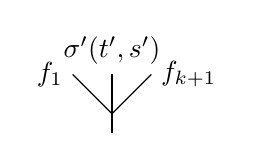
\begin{tikzpicture}[x=0.25cm, y=0.25cm]
				\draw (0,0) -- (0,3);
				\draw (0,1) -- (-2,3);
				\draw (0,1) -- (2,3);
				\draw (0,3) node[above]{$\sigma'(t',s')$};
				\draw (-2,3) node[left]{$f_1$};
				\draw (2,3) node[right]{$f_{k+1}$};				
			\end{tikzpicture}}\right) \text{ where } s=\raisebox{-0.3\height}{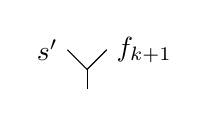
\begin{tikzpicture}[x=0.25cm,y=0.25cm]
			\draw (0,0) -- (0,1);
			\draw (0,1) -- (1,2);
			\draw (0,1) -- (-1,2);
			\draw (-1,2) node[left]{$s'$};
			\draw (1,2) node[right]{$f_{k+1}$};
			\end{tikzpicture}} \\
			&=\begin{tblr}{colspec={cccccccccc},
				cell{2}{1}={r=3,c=3}{c},
				cell{5}{5}={r=3,c=3}{c},
				cell{8}{9}={r=3,c=3}{c}
			}
				 1 & \cdots & 1 & 1 & 1 & \cdots & 1 & 1 & 1 &  \cdots & 1 \\
				F_1 & F_1    & F_1 & \vdots & \vdots & \cdots & \vdots & \vdots & \vdots & \cdots & \vdots \\	
				F_1 & F_1    & F_1 & 1 & 1 & \cdots    & 1 & 1 & 1 & \cdots & 1 \\
				F_1 & F_1    & F_1 & 1 & 1 & \cdots    & 1 & 1 & 1 & \cdots & 1 \\	
				0   & \cdots &  0  & 1 & \Code(\sigma'(t',s')) &   &   & \vdots &\vdots & \cdots & \vdots \\	
				\vdots & \vdots &\vdots& \vdots  & \sigma'(t',s')&   &   & 1 & 1 & \cdots & 1 \\
				0 	& \cdots &  0  & 1 & \sigma'(t',s')&   &   & 1 & 1 & \cdots & 1 \\	
				0 	& \cdots &  0  & 1 & 0			  & \cdots   &  0  & 1 & F_{k+1} & F_{k+1} & F_{k+1} \\
				\vdots	& \cdots &  \vdots  &  \vdots & 0	& \cdots   &  \vdots  & \vdots & F_{k+1} & F_{k+1} & F_{k+1} \\
				0 	& \cdots &  0  & 1 & 0			  & \cdots   &  0  & 1 & F_{k+1} & F_{k+1} & F_{k+1} \\
				0 	& \cdots &  0  & 1 & 0			  & \cdots   &  0  & 1 & 0 & \cdots & 0 \\
				0 	& \cdots &  0  & 0 & 0			  & \cdots   &  0  & 0 & 0 & \cdots & 0 \\
			\end{tblr}
		\end{align*}
		Applying the induction hypothesis as $\RTL(t')+\LTL(s')\leq r$, we have $\Code(\sigma'(t',s'))=\sigma(\Code(t'),\Code(s')).$ Then applying the construction case number $3$ in definition~\ref{defi:quasishuffle_code}, one has:
		\[
		\Code(\sigma(t,s))=\sigma(\Code(t),\Code(s)).
		\]
	\end{description}
	Hence by the induction principle, we have proved the theorem. \qedhere
\end{description}	
\end{proof}
Finally, the map $\Code$ is also linear hence:
\begin{Cor}\label{Cor:iso_codes_trees}
	The $\Code$ map is an isomorphism of tridendriform algebras into its image.
\end{Cor}
\begin{proof}
	To prove this corollary, one just needs to show that $\Code$ is a tridendriform morphism from $(\Sch,\prec,\succ,\cdot)$ into $(\ima(\Code),\prec, \succ, \cdot)$. Let $t,s\in\Sch$ such $t$ has right comb length $k$ and $s$ has left comb length $l$. We show $\Code$ is a morphism for the middle product:
	\begin{align*}
		\Code(t\cdot s)&=\sum_{\substack{\sigma\in\batc(k,l) \\ \sigma^{-1}{\{1\}}=\{1,k+1\}}} \Code(\sigma(t,s)) \\
		&=\sum_{\substack{\sigma\in\batc(k,l) \\ \sigma^{-1}{\{1\}}=\{1,k+1\}}} \sigma(\Code(t),\Code(s)) \\
		&=\Code(t) \cdot\Code(s).
	\end{align*}
	The other cases are similar.
\end{proof}
Now that we are sure the two descriptions are isomorphic, we can get into coding.

\subsection{Short description of the coproduct}\label{sec:coproduct_tree_codes}

We now describe without much details how to interpret the coproduct operation of theorem~\ref{thm:coproduit} for tree codes. Let us remind what is an admissible cut:
\begin{defi}
	Let $t$ be a \Schw{} tree. An \emph{admissible cut} of $t$ is a choice of internal edges in $t$ such that any path from a leaf of the tree to its root meets at most one cut edge. 
	Given a admissible cut $c$, it splits the tree into many connected components removing cut edges. The component with the root of the starting tree is denoted $R^c(t)$ and the other components are denoted $P^c_1(t),\dots, P^c_k(t)$.
	We also consider both elements as admissible cuts:
	\begin{itemize}
		\item the \emph{empty cut} giving $R^c(t)=t$ and $P^c(t)=\unitree$;
		\item the \emph{total cut} giving $R^c(t)=\unitree$ and $P^c(t)=t$.
	\end{itemize}    
\end{defi}
\begin{exam}\label{exam:cut_tree}
	For instance, symbolizing a cut edge by an horizontal line, one has:
	\[
	\raisebox{-0.3\height}{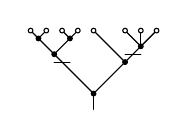
\begin{tikzpicture}[line cap=round,line join=round,>=triangle 45,x=0.2cm,y=0.2cm]
			\draw (0,0)--(0,1);
			% bords de l'arbre
			\draw (0,1)--(-4,5);
			\draw (0,1)--(4,5);
			% bras droit
			\draw (2,3) -- (0,5);
			\draw (3,4) -- (2,5);
			\draw (3,4) -- (3,5);
			\draw (3,4) -- (4,5);
			%bras gauche
			\draw (-3.5,4.5) -- (-3,5);
			\draw (-2.5,3.5) -- (-1,5);
			\draw (-1.5,4.5) -- (-2,5);
			%coupe
			\draw (-2.5,3) -- (-1.5,3);
			\draw (2,3.5) -- (3,3.5);
			% marquages des sommets
			\draw[color=black, fill=white] (-4,5) circle (0.15);
			\draw[color=black, fill=white] (-2,5) circle (0.15);
			\draw[color=black, fill=white] (0,5) circle (0.15);
			\draw[color=black, fill=white] (2,5) circle (0.15);
			\draw[color=black, fill=white] (3,5) circle (0.15);
			\draw[color=black, fill=white] (4,5) circle (0.15);
			\draw[color=black, fill=white] (-3,5) circle (0.15);
			\draw[color=black, fill=white] (-1,5) circle (0.15);
			\filldraw (0,1) circle(0.15);
			\filldraw (-3.5,4.5) circle(0.15);
			\filldraw (-2.5,3.5) circle(0.15);
			\filldraw (-1.5,4.5) circle(0.15);
			\filldraw (3,4) circle(0.15);
			\filldraw (2,3) circle(0.15);
	\end{tikzpicture}} \longrightarrow R^c(t)= \balaisd{} \text{ and } P^c_1(t)=\YY{}, P^c_2(t)=\balais{}.
	\]
\end{exam}

In other words, a cut consists of withdrawing an interval of angles such that both adjacent angles (if they exist) are still living, otherwise the cut is not admissible.
Translating this in term of tree codes, doing a cut of a tree $t$ with $l$ angles is choosing a subset of $\IEM{1}{l}$ where for each integer interval of this subset, when the tree code restricted to this subset is $0$ for the first time at line $i$, the two adjacent columns has a one at line $i$.

\begin{exam}
	For instance, let us consider the tree code of the tree in example~\ref{exam:cut_tree}, the subset of angles corresponds to the cut:
	\[
	\begin{tblr}{colspec={ccccccc},column{1-3}={bg=red!25}, column{6-7}={bg=red!25}
		}
		1 & 1 & 1 & 1 & 1 & 1 & 1 \\
		0 & 1 & 1 & 1 & 1 & 1 & 1 \\
		0 & 1 & 0 & 1 & 1 & 1 & 1 \\
		0 & 0 & 0 & 1 & 1 & 1 & 1 \\
		0 & 0 & 0 & 1 & 1 & 0 & 0 \\
		0 & 0 & 0 & 1 & 0 & 0 & 0 \\
		0 & 0 & 0 & 0 & 0 & 0 & 0
	\end{tblr}  \longleftrightarrow  
	\raisebox{-0.3\height}{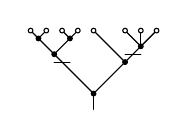
\begin{tikzpicture}[line cap=round,line join=round,>=triangle 45,x=0.2cm,y=0.2cm]
		\draw (0,0)--(0,1);
		% bords de l'arbre
		\draw (0,1)--(-4,5);
		\draw (0,1)--(4,5);
		% bras droit
		\draw (2,3) -- (0,5);
		\draw (3,4) -- (2,5);
		\draw (3,4) -- (3,5);
		\draw (3,4) -- (4,5);
		%bras gauche
		\draw (-3.5,4.5) -- (-3,5);
		\draw (-2.5,3.5) -- (-1,5);
		\draw (-1.5,4.5) -- (-2,5);
		%coupe
		\draw (-2.5,3) -- (-1.5,3);
		\draw (2,3.5) -- (3,3.5);
		% marquages des sommets
		\draw[color=black, fill=white] (-4,5) circle (0.15);
		\draw[color=black, fill=white] (-2,5) circle (0.15);
		\draw[color=black, fill=white] (0,5) circle (0.15);
		\draw[color=black, fill=white] (2,5) circle (0.15);
		\draw[color=black, fill=white] (3,5) circle (0.15);
		\draw[color=black, fill=white] (4,5) circle (0.15);
		\draw[color=black, fill=white] (-3,5) circle (0.15);
		\draw[color=black, fill=white] (-1,5) circle (0.15);
		\filldraw (0,1) circle(0.15);
		\filldraw (-3.5,4.5) circle(0.15);
		\filldraw (-2.5,3.5) circle(0.15);
		\filldraw (-1.5,4.5) circle(0.15);
		\filldraw (3,4) circle(0.15);
		\filldraw (2,3) circle(0.15);
		\end{tikzpicture}}
	\]
\end{exam} 

\section{Implementing the problem} \label{sec:coding}
Thanks to the map denoted $B$, any sequence with $0$'s and $1$'s is identified to an integer the following way:
\[
\forall s\in \{0,1\}^{\star}, B(s)=\sum^{|s|}_{i=0} s_i\cdot 2^i.
\]
Hence, in our code, we will manipulate such sequences as integers. Then, we have to build enumerations and structures needed to perform computations:
\begin{itemize}
	\item enumeration of quasi-shuffles;
	\item class describing \Schw{} trees as sequences of $0$'s and $1$'s;
	\item the $\Omega$ map;
	\item \Schw{} trees enumeration;
	\item the cut coproduct $\Delta$.
\end{itemize}

We do briefs comments about how this code is made. For our objective, we only implemented \Schw{} trees with at most $16$ leaves as they are at this point too much elements ($\num{10463578353}$ trees and $\num{745387038}$ codendriform primitives)  to see anything. We have made the choice to implement this in {\ttfamily C++} to get a faster execution code than one done with {\ttfamily Python} or {\ttfamily \Sage{}}.

%\subsection{The naive implementation}
%
%One naive way to implement this is to use a recursive description given by~\cite{Loday-Ronco} using the grafting operator:
%		\begin{align*}
%	t\prec s&=t^{(1)}\vee \dots \vee \left(t^{(k)}*s\right), \\
%	t\cdot s&=t^{(1)}\vee \dots \vee \left(t^{(k)}* s^{(1)}\right)\vee \dots \vee s^{(l)}, \\
%	t\succ s&=\left(t*s^{(1)}\right)\vee \dots \vee s^{(l)}   ,
%\end{align*}
%where $t=t^{(1)}\vee \dots \vee t^{(k)}$ and $s=s^{(1)}\vee\dots \vee s^{(l)}$, such that $|*t=t=t*|$ for all $t$.
%
%The intuitive algorithm associated to this approach is:
%\begin{lstlisting}[language=Python]
%	def Prod_rec(t1,t2):
%	L1 = Get_subtrees(t1)
%	L2 = Get_subtrees(t2)
%	Left_prod = Graft(L1[0:-1], Prod_rec(L1[-1], L2))
%	Right_prod = Graft( Prod_rec(L1, L2[-1]), L2[0:-1])
%	Middle_prod = Graft(L1[0:-1], Prod_rec(L1[-1],L2[0]) , L2[0:-1])
%	return (Left_prod + Right_prod + Middle_prod)
%\end{lstlisting}
%
%Denote $T(n,m)$ the complexity this algorithm where $n$ and $m$ are respectively the number of leaves of $t_1$ and $t_2.$ Hence, denoting the depth $p_1$ of $t_1$ and $p_2$ of $t_2$, one has:
%\[
%T(n,m) = T\left(\frac{n}{2},m\right) + T\left(n, \frac{m}{2}\right) + T\left(\frac{n}{2},\frac{m}{2}\right) + np_1 +mp_2.
%\]
%Actually, with our encoding, \lstinline[language=Python]|Get_subtrees| needs to read each $n$ column on $p_1$ lines to find subtrees. Let us approximate the complexity where $t_1$ and $t_2$ are both binary trees, have the same number of leaves and at each step the decomposition splits the leaves in two sets of same cardinality. Then denoting $\tilde{T}(n+m)=T(n,m)$, one has:
%\begin{align*}
%	 2 \tilde{T}\left(\frac{3}{4}n\right) + (n-1)\ln_2(n) \leq
%	\tilde{T}(n)\leq 3 \tilde{T}\left(\frac{3}{4}n\right) + (n-1)\ln_2(n).
%\end{align*}
%
%Hence applying the master theorem to compute bounds gives $\left(\ln_{\frac{4}{3}}(2)\approx 2.40, \ln_{\frac{4}{3}}(3)\approx 3.80\right)$ :
%\[
%O(n^{2.40})\leq\tilde{T}(n)\leq O(n^{3.80}).
%\]

\subsection{Quasi-shuffle enumeration}

In the code available on GitHub~\cite{Code}, one can find a procedure \lstinline[language=C++]|Quasishuffle| that returns the list of all quasi-shuffle of a given type $(n,m)$. For this, we use the result from lemma~\ref{lem:Indution_batc} to get an inductive algorithm computing all quasi-shuffles of a given type.

\subsection{The class \Schw{} tree}

We define two classes {\ttfamily \Schw{}Tree} and {\ttfamily \Schw{}Forest} where:
\begin{enumerate}
	\item a tree is list of $16$ integers between $0$ and $2^{16}$. An integer of this lists represents a sequence of zeros and ones needed to build a \Schw{} tree as explained. Hence, its first element is $2^{l+1}-1$ where $l$ is the number of angles of the tree and the last one is $0$. 
	\item a forest is as well a list 
\end{enumerate}

\subsection{The $\Omega$ map}

The map $\Omega$ detailed in theorem~\ref{thm:génération2} is simplified compared to the one given by M.~Ronco~\cite{euleridem} to the price of non-injectivity to get an easier coding.

Let $n\in\NN$ and suppose we know $\Prim_{\Coass}(k)$ for all $n<k$ and $\Prim_{\Codend}(n)$. In order to compute $\Prim_{\Coass}(n)$, we proceed the following way:
\begin{itemize}
	\item we generate an ordered partition of $n=a_1+\dots +a_l$ of length $l$ , denoted $\mathbf{a}$, for all $l\in\IEM{1}{n}$;
	\item if $\mathbf{a}=(n)$, then we apply the identity map;
	\item else according to this partition $\mathbf{a}=(a_1,\dots, a_l)$ with $l\geq 2$, we choose one element $e_i$ in each space $\Prim_{\Coass}(a_i)$ exhaustively and compute $\Omega(a_1\otimes a_2 \otimes \ldots \otimes a_l)$;
	\item we put in memory the results in a matrix, fixing an enumeration of \Schw trees of degree $n$. Columns are indexed by this enumeration and the $i$th row is the $i$th result obtained by this algorithm;
	\item Once the enumeration of ordered partitions is finished, we compute a generating family of the image space of this matrix that we can display.
\end{itemize}
Some computations following this process are given as appendices.

\subsection{\Schw{} enumeration}

Given $n\in\NN$, we provide an enumeration of $\Sch(n)$ thanks to the \emph{snake walk} of a tree since doing this walk tree maps it to a packed word in a bijective way which is easily enumerable the following way

\subsection{The cut coproduct}

The map $\Delta:\K\Sch\rightarrow \K\Sch\otimes \K\Sch$ detailed in theorem~\ref{thm:coproduit} is coded the following way:
\begin{itemize}
	\item for a given tree code $C$
	\item 
	\item 
\end{itemize}




\bibliographystyle{plain}
\bibliography{article.bib}

\end{document}
